\chapter{Eigenvalues of Slabs and Spheres}

In this chapter we verify the correctness and examine the performance of the Rayleigh Quotient Fixed Point methods for one-dimensional media such as slabs and one-dimensional spheres. In slab geometry, the phase space of the neutron transport equation is simplified with only one position variable $x$ and one angular variable $\mu$ defined as the $x$-direction cosine. For slab geometry, the alpha- and $k$-effective eigenvalue neutron transport equations are given by Eq.~\ref{eq:1DAlphaSlab} and Eq.~\ref{eq:1DkSlab}, respectively:

\begin{multline}
\bigg [ \mu \frac{\partial}{\partial x} + \frac{\alpha}{v(E)} + \sigma(x,E) \bigg ] \psi(x,\mu,E) \\ = \frac{\chi(E)}{2} \int_{0}^{\infty} \diff E' \, \nu(E') \sigma_{f}(x,E') \int_{-1}^{1} \diff \mu' \, \psi(x,\mu',E) \\ + \frac{1}{2} \int_{0}^{\infty} \diff E' \, \sigma_{s}(x, E' \rightarrow E) \int_{-1}^{1} \diff \mu' \, \psi(x,\mu',E),
\label{eq:1DAlphaSlab}
\end{multline}
\begin{multline}
\bigg [ \mu \frac{\partial}{\partial x}  + \sigma(x,E) \bigg ] \psi(x,\mu,E) \\ = \frac{1}{k} \frac{\chi(E)}{2} \int_{0}^{\infty} \diff E' \, \nu(E') \sigma_{f}(x,E') \int_{-1}^{1} \diff \mu' \,\psi(x,\mu',E) \\ + \frac{1}{2} \int_{0}^{\infty} \diff E' \, \sigma_{s}(x, E' \rightarrow E) \int_{-1}^{1} \diff \mu' \, \psi(x,\mu',E).
\label{eq:1DkSlab}
\end{multline}

Various homogeneous and heterogeneous slab geometry problems with vacuum boundary conditions were modeled in ARDRA. These slab media problems consist of multiplying and non-multiplying materials with thicknesses $\Delta$. Alpha- and $k$-effective eigenvalues were calculated and the number of transport sweeps compared to various methods such as the critical search method and the power method. To verify the correctness of the Rayleigh Quotient Fixed Point method, the method was compared to various methods such as Green's Function Method (GFM) and Direct Evaluation (DE) and compared to other discrete ordinate neutron transport codes such as PARTISN/DANT.

In one-dimensional spherical geometry, there is only one position variable $r$, the radial position from the center of the sphere, and one angular variable $\mu$ defined as the direction cosine with respect to the radial direction. For spherical geometry, the alpha- and $k$-effective eigenvalue neutron transport equations are given by Eq.~\ref{eq:1DAlphaSphere} and Eq.~\ref{eq:1DkSphere}, respectively:

\begin{multline}
\frac{\mu}{r^{2}} \frac{\partial}{\partial r} \bigg [r^{2} \psi(r,\mu,E) \bigg ] + \frac{1}{r} \frac{\partial}{\partial \mu} \bigg [(1-\mu^{2})\psi(r,\mu,E) \bigg ]+ \sigma(x,E) \psi(r,\mu,E) \\ = \frac{1}{k} \frac{\chi(E)}{2} \int_{0}^{\infty} \diff E' \, \nu(E') \sigma_{f}(r,E') \int_{-1}^{1} \diff \mu' \, \psi(r,\mu',E) \\ + \frac{1}{2} \int_{0}^{\infty} \diff E' \, \sigma_{s}(r, E' \rightarrow E) \int_{-1}^{1} \diff \mu' \, \psi(r,\mu',E),
\label{eq:1DAlphaSphere}
\end{multline}

\begin{multline}
\frac{\mu}{r^{2}} \frac{\partial}{\partial r} \bigg [r^{2} \psi(r,\mu,E) \bigg ] + \frac{1}{r} \frac{\partial}{\partial \mu} \bigg [(1-\mu^{2})\psi(r,\mu,E) \bigg ]+ \bigg [ \frac{\alpha}{v(E)} + \sigma(x,E) \bigg ] \psi(r,\mu,E) \\ = \frac{\chi(E)}{2} \int_{0}^{\infty} \diff E' \, \nu(E') \sigma_{f}(r,E') \int_{-1}^{1} \diff \mu' \, \psi(r,\mu',E) \\ + \frac{1}{2} \int_{0}^{\infty} \diff E' \, \sigma_{s}(r, E' \rightarrow E) \int_{-1}^{1} \diff \mu' \, \psi(r,\mu',E).
\label{eq:1DkSphere}
\end{multline}

For one-dimensional spherical geometry, various homogeneous and heterogeneous spherical problems with vacuum boundary conditions were modeled in ARDRA. Using the same cross-sections for multiplying and non-multiplying materials as the slab media problems, equivalent spherical systems were created using the Davison sphere-equivalence theorem \cite{davison1957neutron} and the alpha-eigenvalue calculated. To verify the correctness of the RQFP for one-dimensional spherical geometry, the method was compared to GFM. Performance of the RQFP for one-dimensional spherical problems was measured by comparing the number of transport sweeps necessary for convergence as compared to the critical search method.

\section{One-Speed Verification for Slab Geometry}

For five one-speed non-multiplying slabs, calculated alpha-eigenvalues were benchmarked to the GFM \cite{kornreich_timeeigenvalue_2005}, described in Section~\ref{sec:CalcAlpha}. For these sets of problems, the neutron speed was set to $v = 1$ cm/s and the total cross section set to unity $\sigma = 1$ cm$^{-1}$. The slabs were purely scattering (Table~\ref{table:Betzler}). Problem thicknesses $\Delta$ were in mean free paths (mfps).

\begin{table}[H]
    \centering
    \caption{Non-Multiplying Homogeneous Slab Cross Sections (cm$^{-1}$)}
\label{table:Betzler}
    \begin{tabular}{*4c}
        \toprule
	$\sigma$ & $\nu \sigma_{f}$ & $\sigma_{s}$  & $v$ [cm/s] \\ 
        \midrule
	1.0 & 0.0 & 1.0 & 1.0 \\
        \bottomrule
    \end{tabular}
\end{table}

For multiplying media, 22 one-speed slabs of varying thickness $\Delta$ were examined and the Rayleigh Quotient Fixed Point method calculated alpha-eigenvalues were benchmarked to the GFM. The total cross section was set to unity and the slab neutron multiplication set to $\nu \sigma_{f} = 0.25$. The scattering cross section was set to $\sigma_{s} = 0.9$ cm$^{-1}$ (Table~\ref{table:Betzler2}).

\begin{table}[H]
    \centering
    \caption{Multiplying Homogeneous Slab Cross Sections (cm$^{-1}$)}
\label{table:Betzler2}
    \begin{tabular}{*5c}
        \toprule
	$\sigma$ & $\nu \sigma_{f}$ & $\sigma_{s}$ & $v$ [cm/s] \\ 
        \midrule
	1.0 & 0.25 & 0.9 & 1.0 \\
        \bottomrule
    \end{tabular}
\end{table}

Five one-speed heterogeneous slab problems consisting of two materials were examined and the Rayleigh Quotient Fixed Point method calculated alpha-eigenvalues compared to the GFM, direct evaluation (DE) \cite{modak_simple_2003}, and DANT/PARTISN \cite{alcouffe2005partisn}. With a fixed maximum medium width, material slabs of thickness $\Delta$ with cross sections as seen in Table~\ref{table:BetzlerHetero} were alternated until reaching the maximum fixed width. The impact of material widths on the alpha-eigenvalue was examined for this non-multiplying medium.

\begin{table}[H]
    \centering
    \caption{Non-Multiplying Heterogeneous Slab Material Cross Sections (cm$^{-1}$)}
\label{table:BetzlerHetero}
    \begin{tabular}{*6c}
        \toprule
	Material & $\sigma$ & $\nu \sigma_{f}$ & $\sigma_{s}$ & $v_{g}$ [cm/s] \\ 
        \midrule
	1 & 10.0 & 0.0 & 10.0 & 1.0 \\
	2 & 10.0 & 0.0 & 9.0 & 1.0 \\
	Homogeneous & 10.0 & 0.0 & 9.5 & 1.0 \\
        \bottomrule
    \end{tabular}
\end{table}

A two-region multiplying slab was examined with material properties as seen in Table~\ref{table:BetzlerHeteroMult}. The problem consisted of a 1.5 mfp region on the right and a 1.0 mfp region to the left. Both materials were multiplying and the system was supercritical \cite{kornreich_greens_1997}.

\begin{table}[H]
    \centering
    \caption{Multiplying Heterogeneous Slab Material Cross Sections (cm$^{-1}$)}
\label{table:BetzlerHeteroMult}
    \begin{tabular}{*6c}
        \toprule
	Material & $\sigma$ & $\nu \sigma_{f}$ & $\sigma_{s}$ & $v_{g}$ [cm/s] \\ 
        \midrule
	1 & 1.0 & 0.6 & 0.9 & 1.0 \\
	2 & 1.0 & 0.3 & 0.2 & 1.0 \\ 
        \bottomrule
    \end{tabular}
\end{table}

Four one-speed five region slab problems consisting of fuel, moderator, and absorber materials were examined and the Rayleigh Quotient Fixed Point method alpha-eigenvalue compared to the GFM. The leftmost fuel pin width was allowed to vary (see Figure~\ref{fig:FiveRegionProblem}).The alpha-eigenvalue was calculated for different fuel width thicknesses with the fuel having $\nu \sigma_{f} = 0.3$ or $0.7$. Cross sections for the three materials are seen in Table~\ref{table:BetzlerFive}.

\begin{table}[H]
    \centering
    \caption{Five Region Slab Material Cross Sections (cm$^{-1}$)}
\label{table:BetzlerFive}
    \begin{tabular}{*6c}
        \toprule
	Material & $\sigma$ & $\nu \sigma_{f}$ & $\sigma_{s}$ & $v_{g}$ [cm/s] \\ 
        \midrule
	Fuel & 1.0 & 0.3/0.7 & 0.8 & 1.0 \\
	Moderator & 1.0 & 0.0 & 0.8 & 1.0 \\ 
	Absorber & 1.0 & 0.0 & 0.1 & 1.0 \\ 
        \bottomrule
    \end{tabular}
\end{table}

\subsection{Non-Multiplying Homogeneous Slabs with Isotropic Scattering}
For the one-speed, purely-scattering, homogeneous slabs of thicknesses $\Delta = 1.0$ to $\Delta = 25.0$ mfp with cross sections shown in Table~\ref{table:Betzler}, the Rayleigh Quotient Fixed Point method showed good agreement with the GFM (Table~\ref{table:CompHomogScatt}). For diamond difference discretization ($M = 500$ cells) and S$_{64}$ discrete ordinates quadrature ($L = 64$), the subcritical alpha-eigenvalues matched within less than 0.1\% relative error. $500$ spatial cells and $64$ angular quadrature points were selected to guarantee the positivity of the flux solution for all slab widths. The greatest discrepancy between the two methods was for $\Delta = 1.0$ mfp. In \cite{kornreich_timeeigenvalue_2005}, it is noted that the GFM has difficulty obtaining obtaining accurate eigenvalue results for thin slabs. As the slab thickness increases, the number of transport sweeps necessary to converge the alpha-eigenvalue to a tolerance of $10^{-12}$ increases. However, the relative error between RQFP and the GFM decreases. For problems without any multiplication, the $k$-effective eigenvalue is not defined.

\begin{table*}[!htbp]
\centering\ra{1.3}
\caption{Comparison of RQFP- and GFM-calculated Alpha-Eigenvalues for a Homogeneous Scattering Slab}
\label{table:CompHomogScatt}
\begin{tabular}{@{}cccc@{}}\toprule
& \multicolumn{3}{c}{Alpha-Eigenvalue/Percent Relative Error} \\
\cmidrule{2-4} $\Delta$ & RQFP & GFM & \% Relative Error \\
\midrule
%$\Delta$\\
1 & $-6.08420 \times 10^{-1}$ & $-6.08072 \times 10^{-1}$ & 0.057189 \\ 
5 & $-8.10966 \times 10^{-2}$ & $-8.10933 \times 10^{-2}$ & 0.004113 \\ 
10 & $-2.53506 \times 10^{-2}$ & $-2.53500 \times 10^{-2}$ & 0.002349 \\ 
20 & $-7.18015 \times 10^{-3}$ & $-7.17962 \times 10^{-3}$ & 0.007358 \\ 
25 & $-4.71736 \times 10^{-3}$ & $-4.71722 \times 10^{-3}$ & 0.002966 \\ 
\bottomrule
\multicolumn{4}{l}{$M = 500$, $L = 64$, Tolerance = $10^{-12}$} \\
\end{tabular}
\end{table*}

\subsection{Multiplying Homogeneous Slab}

For the material cross sections shown in Table~\ref{table:Betzler2}, one-speed homogeneous multiplying slabs of thicknesses of thickness $\Delta = 1.0$ to $\Delta = 50.0$ mfp showed good agreement between RQFP and the GFM with the exception of thin slabs. For thin slabs of up to width $\Delta = 1.0$ mfp, percent relative error was substantial. This is caused by the difficulty of numerically determining the alpha-eigenvalues for thin slabs by the GFM. As the slab thickness increased, agreement was substantially better (Table~\ref{table:CompHomogMult}). 

The alpha-eigenvalue RQFP was compared to the critical search method (Table~\ref{table:CompMultSweeps}). The RQFP method substantially outperformed the critical search method in all cases and was able to converge subcritical alpha-eigenvalues that the critical search method could not determine. As the system became more supercritical, the number of transport sweeps necessary to converge increased for both methods. For the most supercritical slab ($\Delta = 50.0$ mfp), the number of sweeps necessary for the RQFP method to converge was less than the number of transport sweeps necessary for critical search to converge for the $\Delta = 4.0$ mfp case. Since the RQFP method requires no intermediate $k$-effective eigenvalue calculations, the method substantially reduced the number of transport sweeps necessary as there was no need to do multiple $k$-effective eigenvalue calculations to bracket the alpha-eigenvalue.

For the one-speed homogeneous multiplying slabs of varying thickness, the $k$-effective eigenvalue RQFP method was compared to the power method with the fission norm update (Table~\ref{table:CompMultSweepsK}). It was seen that the number of transport sweeps for convergence increased as the $k$-effective eigenvalue increased. The RQFP method required far more sweeps than the power method, up to a factor of five. Underperformance of the RQFP method for these particular $k$-effective problems is believed to be caused by flattening of the fundamental angular flux mode. As the system thickness is increases, the flux profile is flattened but higher flux modes take longer to decay.

\begin{table*}[!htbp]
\centering\ra{1.3}
\caption{Comparison of RQFP- and GFM-calculated Alpha-Eigenvalues for a Homogeneous Scattering Multiplying Slab}
\label{table:CompHomogMult}
\begin{tabular}{@{}cccc@{}}\toprule
& \multicolumn{3}{c}{Alpha-Eigenvalue/Percent Relative Error} \\
\cmidrule{2-4} $\Delta$ & RQFP & GFM & \% Relative Error \\
\midrule
%$\Delta$\\
%0.25 & $-1.15480 \times 10^{0}$ & $-9.90300 \times 10^{-1}$ & 16.611352 \\ 
%0.30 & $-1.06633 \times 10^{0}$ & $-9.74300 \times 10^{-1}$ & 9.446240 \\ 
0.25 & $-1.15480 $ & $-9.90300 \times 10^{-1}$ & 16.611352 \\ 
0.30 & $-1.06633 $ & $-9.74300 \times 10^{-1}$ & 9.446240 \\ 
0.35 & $-9.98584 \times 10^{-1}$ & $-9.49350 \times 10^{-1}$ & 5.186069 \\ 
0.40 & $-9.42114 \times 10^{-1}$ & $-9.17000 \times 10^{-1}$ & 2.738758 \\ 
0.45 & $-8.91833 \times 10^{-1}$ & $-8.79460 \times 10^{-1}$ & 1.406940 \\ 
0.50 & $-8.44920 \times 10^{-1}$ & $-8.38790 \times 10^{-1}$ & 0.730822 \\ 
0.75 & $-6.34756 \times 10^{-1}$ & $-6.34060 \times 10^{-1}$ & 0.109818 \\ 
1 & $-4.69398 \times 10^{-1}$ & $-4.69160 \times 10^{-1}$ & 0.050762 \\ 
2 & $-1.36335 \times 10^{-1}$ & $-1.36310 \times 10^{-1}$ & 0.018335 \\ 
3 & $-1.39888 \times 10^{-2}$ & $-1.39790 \times 10^{-2}$ & 0.070397 \\ 
4 & $4.36998 \times 10^{-2}$ & $4.37050 \times 10^{-2}$ & 0.011811 \\ 
5 & $7.54667 \times 10^{-2}$ & $7.54690 \times 10^{-2}$ & 0.003096 \\ 
6 & $9.48296 \times 10^{-2}$ & $9.48310 \times 10^{-2}$ & 0.001470 \\ 
7 & $1.07508 \times 10^{-1}$ & $1.07510 \times 10^{-1}$ & 0.002137 \\ 
8 & $1.16263 \times 10^{-1}$ & $1.16260 \times 10^{-1}$ & 0.002344 \\ 
9 & $1.22563 \times 10^{-1}$ & $1.22560 \times 10^{-1}$ & 0.002390 \\ 
10 & $1.27248 \times 10^{-1}$ & $1.27250 \times 10^{-1}$ & 0.001492 \\ 
15 & $1.39126 \times 10^{-1}$ & $1.39130 \times 10^{-1}$ & 0.002605 \\ 
20 & $1.43649 \times 10^{-1}$ & $1.43650 \times 10^{-1}$ & 0.000663 \\ 
30 & $1.47066 \times 10^{-1}$ & $1.47070 \times 10^{-1}$ & 0.002483 \\ 
40 & $1.48317 \times 10^{-1}$ & $1.48320 \times 10^{-1}$ & 0.001982 \\ 
50 & $1.48910 \times 10^{-1}$ & $1.48910 \times 10^{-1}$ & 0.000004 \\ 
\bottomrule
\multicolumn{4}{l}{$M = 500$, $L = 64$, Tolerance = $10^{-12}$} \\
\end{tabular}
\end{table*}


\begin{table}[!htbp]
	\caption{Transport Sweep Comparisons for Homogeneous Multiplying Slabs}
	\resizebox{0.94\textwidth}{!}{%
	\begin{subtable}[!htbp]{1.0\textwidth}
	\centering\ra{1.3}
	\begin{tabular}{@{}cccccc@{}}\toprule
	& \multicolumn{2}{c}{Transport Sweeps} & & \multicolumn{2}{c}{Transport Sweeps} \\
	\cmidrule{2-3} \cmidrule{5-6} $\Delta$ & RQFP & Critical Search \quad &  \Delta & RQFP & Critical Search\\
	\midrule
	%$\Delta$\\
%	4 & 56 & 21044 & 10 & 166 & 78002\\ 
%	5 & 70 & 33036 & 15 & 308 & 89627 \\
%	6 & 85 & 44655 & 20 & 495 & 97267 \\
%	7 & 103 & 55242 & 30 & 1002 & 98087 \\ 
%	8 & 122 & 63851 & 40 & 1682 & 106055 \\ 
%	9 & 143 & 71181 & 50 & 2530 & 113189 \\
	0.25 & 95 & * & 5 & 70 & 33036 \\
	0.30 & 98 & * & 6 & 85 & 44655 \\
	0.35 & 99 & * & 7 & 103 & 55242 \\
	0.40 & 95 & * & 8 & 122 & 63851 \\
	0.45 & 91 & * & 9 & 143 & 71181 \\
	0.50 & 84 & * & 10 & 166 & 78002 \\
	0.75 & 52 & * & 15 & 308 & 89627 \\
	1 & 34 & * & 20 & 495 & 97267 \\
	2 & 32 & * & 30 & 1002 & 98087 \\
	3 & 43 & * & 40 & 1682 & 106055 \\ 
	4 & 56 & 21044 & 50 & 2530 & 113189 \\
	\bottomrule
	\multicolumn{6}{l}{*Did Not Converge} \\
	\end{tabular}
	\caption{Alpha-Eigenvalue: Comparison of RQFP and Critical Search Sweeps}
	\label{table:CompMultSweeps}
	\end{subtable}}
	\vspace{0.25cm}
	\resizebox{0.95\textwidth}{!}{%
	\begin{subtable}[!htbp]{1.0\textwidth}
	\centering\ra{1.3}
	\begin{tabular}{@{}cccccc@{}}\toprule
	& \multicolumn{2}{c}{Transport Sweeps} & & \multicolumn{2}{c}{Transport Sweeps} \\
	\cmidrule{2-3} \cmidrule{5-6} $\Delta$ & RQFP & Power Method \quad &  \Delta & RQFP & Power Method\\
	\midrule
	%$\Delta$\\
%	1 & 23 & 22 & 20 & 445 & 115\\ 
%	2 & 33 & 27 & 25 & 650 & 156 \\
%	4 & 54 & 34 & 30 & 892 & 206 \\
%	5 & 67 & 37 & 40 & 1490 & 328 \\ 
%	10 & 154 & 55 & 50 & 2235 & 481 \\ 
%	15 & 280 & 81 &  &  &  \\
	0.25 & 16 & 17 & 5 & 67 & 37 \\
	0.30 & 16 & 17 & 6 & 81 & 40 \\
	0.35 & 17 & 18 & 7 & 97 & 44 \\
	0.40 & 18 & 19 & 8 & 115 & 47 \\
	0.45 & 18 & 19 & 9 & 133 & 51 \\
	0.50 & 19 & 19 & 10 & 154 & 55 \\
	0.75 & 21 & 21 & 15 & 280 & 81 \\
	1 & 23 & 22 & 20 & 445 & 115 \\
	2 & 33 & 27 & 30 & 892 & 206 \\
	3 & 43 & 31 & 40 & 1490 & 238 \\
	4 & 54 & 34 & 50 & 2235 & 481 \\
	\bottomrule
	\multicolumn{6}{l}{$M = 500$, $L = 64$, Tolerance = $10^{-12}$} \\
	\end{tabular}
	\caption{$k$-Effective: Comparison of RQFP and Power Method Transport Sweeps}
	\label{table:CompMultSweepsK}
	\end{subtable}}
\end{table}

%\begin{table*}[t]
%\centering\ra{1.3}
%\caption{Alpha-Eigenvalue: Comparison of RQFP and Critical Search Sweeps for Homogeneous Multiplying Slabs}
%\label{table:CompMultSweeps}
%\begin{tabular}{@{}cccccc@{}}\toprule
%& \multicolumn{2}{c}{Transport Sweeps} & & \multicolumn{2}{c}{Transport Sweeps} \\
%\cmidrule{2-3} \cmidrule{5-6} $\Delta$ & RQFP & Critical Search \quad &  \Delta & RQFP & Critical Search\\
%\midrule
%%$\Delta$\\
%4 & 56 & 21044 & 10 & 166 & 78002\\ 
%5 & 70 & 33036 & 15 & 308 & 89627 \\
%6 & 85 & 44655 & 20 & 495 & 97267 \\
%7 & 103 & 55242 & 30 & 1002 & 98087 \\ 
%8 & 122 & 63851 & 40 & 1682 & 106055 \\ 
%9 & 143 & 71181 & 50 & 2530 & 113189 \\
%\bottomrule
%\multicolumn{6}{l}{$M = 500$, $L = 64$, Tolerance = $10^{-12}$} \\
%\end{tabular}
%\end{table*}
%
%\begin{table*}[t]
%\centering\ra{1.3}
%\caption{$k$-Effective: Comparison of RQFP and Power Method Transport Sweeps for Homogeneous Multiplying Slabs}
%\label{table:CompMultSweepsK}
%\begin{tabular}{@{}cccccc@{}}\toprule
%& \multicolumn{2}{c}{Transport Sweeps} & & \multicolumn{2}{c}{Transport Sweeps} \\
%\cmidrule{2-3} \cmidrule{5-6} $\Delta$ & RQFP & Power Method \quad &  \Delta & RQFP & Power Method\\
%\midrule
%%$\Delta$\\
%1 & 23 & 22 & 20 & 445 & 115\\ 
%2 & 33 & 27 & 25 & 650 & 156 \\
%4 & 54 & 34 & 30 & 892 & 206 \\
%5 & 67 & 37 & 40 & 1490 & 328 \\ 
%10 & 154 & 55 & 50 & 2235 & 481 \\ 
%15 & 280 & 81 &  &  &  \\
%\bottomrule
%\multicolumn{6}{l}{$M = 500$, $L = 64$, Tolerance = $10^{-12}$} \\
%\end{tabular}
%\end{table*}
%
\clearpage
\subsection{Multiplying Homogeneous Slabs with Anisotropic Scattering}

\textbf{Sood Criticality Benchmark Problems 32-35}: Four one-group critical slab problems with anisotropic scattering were examined to demonstrate the performance of the Rayleigh Quotient Fixed Point method. For each set of cross sections in Table~\ref{table:SoodPUAniso}, two distinct problems with P1 or P2 scattering were considered. In these problems, the scattering kernel is non-negative. All problems were exactly critical with the critical half-width, $r_{c}$, defined in Figure~\ref{fig:SlabCritWidth}, given in Table~\ref{table:SlabAniso}.

For the alpha-eigenvalue problems, the RQFP-calculated alpha-eigenvalues are seen in Table~\ref{table:CompAnisoSweepAlpha}. All problems were slightly subcritical but within $10^{-5}$ of the actual alpha-eigenvalue of zero. The RQFP method took 22-26 transport sweeps to converge the eigenvector $\ell_{2}$ norm residual to $10^{-12}$ (Table~\ref{table:CompAnisoSweepAlpha}). Since the problems were too close to critical and slightly subcritical, the critical search method could not converge the problem.

For $k$-effective eigenvalue problems, the RQFP-calculated eigenvalues are seen in Table~\ref{table:CompAnisoSweepk} The problems had a calculated $k$-effective eigenvalue slightly below the true eigenvalue of one. The RQFP method took 22-26 transport sweeps to converge the $\ell_{2}$ norm eigenvector residual to $10^{-12}$. The power method with the fission source update required 3-4 transport sweeps less than the RQFP method for all problems.

\begin{figure}[!htbp]
	\centering
	\begin{tikzpicture}[text centered]
    \begin{scope}[thick,font=\Large]

    \draw [-] (-2.5,-3) -- (-2.5,3) {};
%    \draw [-] (2.5,-3) -- (0.5,3) {};
    
    \draw [dashed] (0.0,-4) -- (0,4) {};
    \draw (2.5,-3) -- (2.5,3) {};
    
    \draw [->] (0,0) -- (2.5,0) node [align=center] at (1.25,0.3) {$r_{c}$};

    \end{scope}
\end{tikzpicture}
	\caption{Critical Width of Slab}
	\label{fig:SlabCritWidth}
\end{figure}

\begin{table}[!htbp]
	\caption{Plutonium Cross Sections with Anisotropic Scattering for Critical Slab Problems (cm$^{-1}$) \cite{sood2003analytical}}
	\label{table:SoodPUAniso}
	\centering\ra{1.3}
    \begin{tabular}{*6c}
        \toprule
	Cross Section Set & $\sigma$ & $\nu \sigma_{f}$ & $\sigma_{s0}$  & $\sigma_{s1}$ & $v$ [cm/s] \\ 
        \midrule
	PUa & 0.32640 & 0.176256 & 0.248064 & 0.042432 & 1 \\
	PUb & 0.32640 & 0.176256 & 0.248064 & 0.212160 & 1 \\
        \bottomrule
    \end{tabular}
\end{table}

\begin{table}[!htbp]
	\caption{Calculated Eigenvalues and Transport Sweep Comparisons for Critical Slab Problems with Anisotropic Scattering in \cite{sood2003analytical}}
	\label{table:SlabAniso}
	\begin{subtable}[!htbp]{1.0\textwidth}
	\centering\ra{1.3}
	\begin{tabular}{@{}ccccc@{}}\toprule
	& & & \multicolumn{2}{c}{Transport Sweeps} \\
	\cmidrule{4-5} Cross Section Set & $r_{c}$ [cm] & Calculated $\alpha$ [s$^{-1}$] & RQFP & Critical Search\\
	\midrule
	PUa-P1 Scattering & 0.77032 & $-3.50639 \times 10^{-5}$ & 24 & *\\
	PUb-P1 Scattering & 0.76378 & $-6.16666 \times 10^{-5}$ & 26 & * \\
	PUa-P2 Scattering & 0.79606 & $-5.29475 \times 10^{-5}$ & 24 & *\\
	PUb-P2 Scattering & 0.78396 & $-2.72628 \times 10^{-5}$ & 22 & * \\
	\bottomrule
	\multicolumn{5}{l}{*Did Not Converge} \\
	\end{tabular}
	\caption{Alpha-Eigenvalue: Comparison of RQFP and Critical Search Transport Sweeps}
	\label{table:CompAnisoSweepAlpha}
	\end{subtable}%
	\vspace{0.25cm}
	\begin{subtable}[!htbp]{1.0\textwidth}
	\centering\ra{1.3}
	\begin{tabular}{@{}ccccc@{}}\toprule
	& & & \multicolumn{2}{c}{Transport Sweeps} \\
	\cmidrule{4-5} Cross Section Set & $r_{c}$ [cm] & Calculated $k_{\text{eff}}$ & RQFP & Power Method\\
	\midrule
	PUa-P1 Scattering & 0.77032 & 0.99995 & 25 & 22 \\
	PUb-P1 Scattering & 0.76378 & 0.99991 & 26 & 24 \\
	PUa-P2 Scattering & 0.79606 & 0.99993 & 22 & 18 \\
	PUb-P2 Scattering & 0.78396 & 0.99996 & 24 & 21 \\
	\bottomrule%	
	\multicolumn{5}{l}{$M = 500$, $L = 64$, Tolerance = $10^{-12}$} \\
	\end{tabular}
	\caption{$k$-Effective: Comparison of RQFP and Power Method Transport Sweeps}
	\label{table:CompAnisoSweepk}
	\end{subtable}
\end{table}

\clearpage
\subsection{Heterogeneous Slabs}

\textbf{Problem 6.1.3.1-Non-multiplying Heterogeneous Slab}: For the subcritical heterogeneous medium shown in Figure~\ref{fig:HeteroSlabDomain}, five problems were constructed by varying the grain sizes of alternating slabs consisting of materials with the cross sections shown in Table~\ref{table:BetzlerHetero}. The maximum width of the domain was fixed at 10.0 mfp as in \cite{kornreich_timeeigenvalue_2005}. Grain sizes of 0.5, 1, 2.5, and 5 mfp were examined and their alpha-eigenvalue calculated by the RQFP method and compared to the GFM. One last case consisting of a homogenized material was considered. In all cases, the RQFP method showed good agreement with DANT/PARTISN (Table~\ref{AlphaDANT}), Green's Function Method (Table~\ref{AlphaGFM}), and Direct Evaluation (Table~\ref{AlphaDE}) with percent relative error within 0.15\%. The number of transport sweeps required to obtain the eigenvalue and eigenvector increased as the problem approached critical and the number of regions increased. The scalar fluxes for the four heterogeneous region problems can be seen in Figure~\ref{fig:GrainScalarFlux}

\begin{figure}[!htbp]
	\centering
	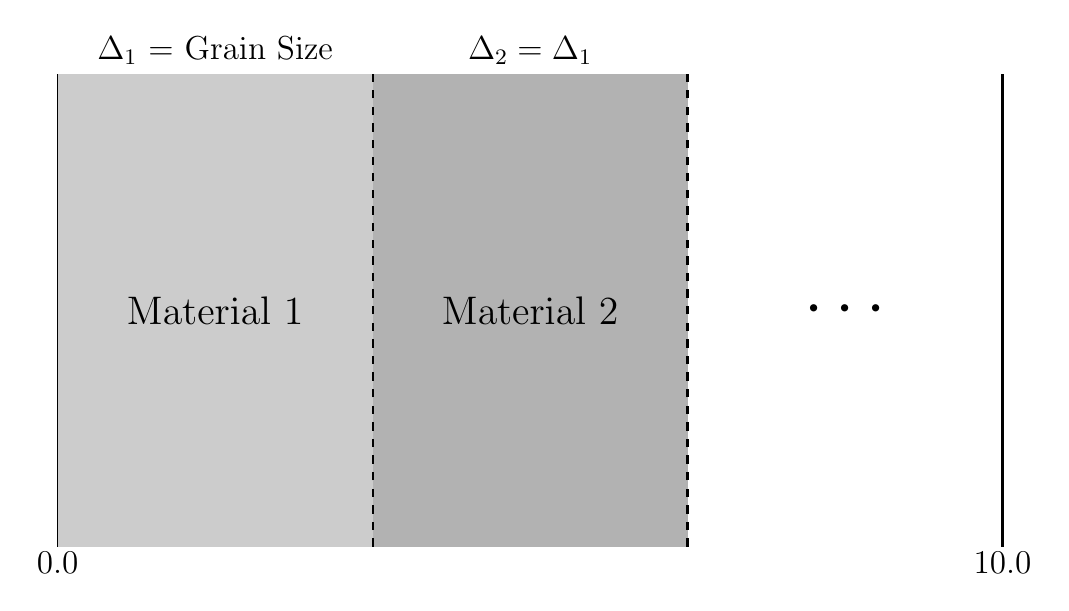
\begin{tikzpicture}
    \begin{scope}[thick,font=\scriptsize]

    \draw [-] (-3,-3) -- (-3,3) {};
    \draw [-] (9,-3) -- (9,3) {};
    
    \draw node at (-3,-3.2) {\large $0.0$};
    \draw node at (9,-3.2) {\large $10.0$};
    
    \fill[fill=black!20] (-3,-3) rectangle (1,3);
    \fill[fill=black!30] (1,-3) rectangle (5,3);
    
    \draw [dashed] (1,-3) -- (1,3) {};
    \draw [dashed] (5,-3) -- (5,3) {};
    
    \draw node at (-1,0) {\Large Material 1};
    \draw node at (3,0) {\Large Material 2};
    \draw node at (7,0) {\Huge{$\cdots$}};
    
    \draw node at (-1,3.3) {\large $\Delta_{1}$ = Grain Size}; 
    \draw node at (3,3.3) {\large $\Delta_{2} = \Delta_{1}$};

    \end{scope}
\end{tikzpicture}
	\caption{Heterogeneous Slab Benchmark Problem Domain \cite{kornreich_timeeigenvalue_2005}}
	\label{fig:HeteroSlabDomain}
\end{figure}

\begin{table}[!htbp]
	\caption{Comparison of RQFP-calculated eigenvalues to various methods for multi-region scattering slab ($M = 500$, $L = 64$, Tolerance = $10^{-12}$)}
	\label{table:RQ_DE_DANT_GFM}
	\begin{subtable}[!htbp]{1.0\textwidth}
	\centering\ra{1.3}
	\begin{tabular}{@{}lccc@{}}\toprule
	& \multicolumn{3}{c}{Alpha-Eigenvalue/Percent Relative Error} \\
	\cmidrule{2-4} Grain Size & RQFP & DANT/PARTISN & \% Relative Error \\
	\midrule
	5 (2 slabs) & $-5.51528 \times 10^{-1}$ & $-5.50813 \times 10^{-1}$ & 0.129782 \\ 
	2.5 (4 slabs) & $-7.03144 \times 10^{-1}$ & $-7.03134 \times 10^{-1}$ & 0.001470 \\ 
	1 (10 slabs) & $-7.48808 \times 10^{-1}$ & $-7.48793 \times 10^{-1}$ & 0.001942 \\ 
	0.5 (20 slabs) & $-7.57221 \times 10^{-1}$ & $-7.57199 \times 10^{-1}$ & 0.002882 \\ 
	0 (homogeneous) & $-7.63513 \times 10^{-1}$ & $-7.63507 \times 10^{-1}$ & 0.000848 \\ 
	\bottomrule
	%\multicolumn{4}{l}{$M = 500$, $L = 64$, Tolerance = $10^{-12}$} \\
	\end{tabular}
	\caption{Comparison of RQFP- and DANT/PARTISN-calculated alpha-eigenvalues}
	\label{AlphaDANT}
	\end{subtable}%
	\vspace{0.25cm}
	\begin{subtable}[!htbp]{1.0\textwidth}
	\centering\ra{1.3}
	\begin{tabular}{@{}lccc@{}}\toprule
	& \multicolumn{3}{c}{Alpha-Eigenvalue/Percent Relative Error} \\
	\cmidrule{2-4} Grain Size & RQFP & GFM & \% Relative Error \\
	\midrule
	5 (2 slabs) & $-5.51528 \times 10^{-1}$ & $-5.50812 \times 10^{-1}$ & 0.129964 \\ 
	2.5 (4 slabs) & $-7.03144 \times 10^{-1}$ & $-7.03133 \times 10^{-1}$ & 0.001612 \\ 
	1 (10 slabs) & $-7.48808 \times 10^{-1}$ & $-7.48792 \times 10^{-1}$ & 0.002075 \\ 
	0.5 (20 slabs) & $-7.57221 \times 10^{-1}$ & $-7.57198 \times 10^{-1}$ & 0.003014 \\ 
	0 (homogeneous) & $-7.63513 \times 10^{-1}$ & $-7.63507 \times 10^{-1}$ & 0.000848 \\ 
	\bottomrule
	%\multicolumn{4}{l}{$M = 500$, $L = 64$, Tolerance = $10^{-12}$} \\
	\end{tabular}
	\caption{Comparison of RQFP- and GFM-calculated alpha-eigenvalues}
	\label{AlphaGFM}
	\end{subtable}%
	\vspace{0.25cm}
	\begin{subtable}[!htbp]{1.0\textwidth}
	\centering\ra{1.3}
	\begin{tabular}{@{}lccc@{}}\toprule
	& \multicolumn{3}{c}{Alpha-Eigenvalue/Percent Relative Error} \\
	\cmidrule{2-4} Grain Size & RQFP & GFM & \% Relative Error \\
	\midrule
	5 (2 slabs) & $-5.51528 \times 10^{-1}$ & $-5.50812 \times 10^{-1}$ & 0.129964 \\ 
	2.5 (4 slabs) & $-7.03144 \times 10^{-1}$ & $-7.03133 \times 10^{-1}$ & 0.001612 \\ 
	1 (10 slabs) & $-7.48808 \times 10^{-1}$ & $-7.48792 \times 10^{-1}$ & 0.002075 \\ 
	0.5 (20 slabs) & $-7.57221 \times 10^{-1}$ & $-7.57198 \times 10^{-1}$ & 0.003014 \\ 
	0 (homogeneous) & $-7.63513 \times 10^{-1}$ & $-7.63507 \times 10^{-1}$ & 0.000848 \\ 
	\bottomrule
	%\multicolumn{4}{l}{$M = 500$, $L = 64$, Tolerance = $10^{-12}$} \\
	\end{tabular}
	\caption{Comparison of RQFP- and DE-calculated alpha-eigenvalues}
	\label{AlphaDE}
	\end{subtable}
\end{table}

%\begin{table*}
%\centering\ra{1.3}
%\caption{Comparison of RQFP- and DANT/PARTISN-calculated alpha-eigenvalues for a multi-region scattering slab}
%\label{AlphaDANT}
%\begin{tabular}{@{}lccc@{}}\toprule
%& \multicolumn{3}{c}{Alpha-Eigenvalue/Percent Relative Error} \\
%\cmidrule{2-4} Grain Size & RQFP & DANT/PARTISN & \% Relative Error \\
%\midrule
%5 (2 slabs) & $-5.51528 \times 10^{-1}$ & $-5.50813 \times 10^{-1}$ & 0.129782 \\ 
%2.5 (4 slabs) & $-7.03144 \times 10^{-1}$ & $-7.03134 \times 10^{-1}$ & 0.001470 \\ 
%1 (10 slabs) & $-7.48808 \times 10^{-1}$ & $-7.48793 \times 10^{-1}$ & 0.001942 \\ 
%0.5 (20 slabs) & $-7.57221 \times 10^{-1}$ & $-7.57199 \times 10^{-1}$ & 0.002882 \\ 
%0 (homogeneous) & $-7.63513 \times 10^{-1}$ & $-7.63507 \times 10^{-1}$ & 0.000848 \\ 
%\bottomrule
%\multicolumn{4}{l}{$M = 500$, $L = 64$, Tolerance = $10^{-12}$} \\
%\end{tabular}
%\end{table*}
%
%\begin{table*}
%\centering\ra{1.3}
%\caption{Comparison of RQFP- and GFM-calculated alpha-eigenvalues for a multi-region scattering slab}
%\label{AlphaGFM}
%\begin{tabular}{@{}lccc@{}}\toprule
%& \multicolumn{3}{c}{Alpha-Eigenvalue/Percent Relative Error} \\
%\cmidrule{2-4} Grain Size & RQFP & GFM & \% Relative Error \\
%\midrule
%5 (2 slabs) & $-5.51528 \times 10^{-1}$ & $-5.50812 \times 10^{-1}$ & 0.129964 \\ 
%2.5 (4 slabs) & $-7.03144 \times 10^{-1}$ & $-7.03133 \times 10^{-1}$ & 0.001612 \\ 
%1 (10 slabs) & $-7.48808 \times 10^{-1}$ & $-7.48792 \times 10^{-1}$ & 0.002075 \\ 
%0.5 (20 slabs) & $-7.57221 \times 10^{-1}$ & $-7.57198 \times 10^{-1}$ & 0.003014 \\ 
%0 (homogeneous) & $-7.63513 \times 10^{-1}$ & $-7.63507 \times 10^{-1}$ & 0.000848 \\ 
%\bottomrule
%\multicolumn{4}{l}{$M = 500$, $L = 64$, Tolerance = $10^{-12}$} \\
%\end{tabular}
%\end{table*}
%
%\begin{table*}
%\centering\ra{1.3}
%\caption{Comparison of RQFP- and DE-calculated alpha-eigenvalues for a multi-region scattering slab}
%\label{AlphaDE}
%\begin{tabular}{@{}lccc@{}}\toprule
%& \multicolumn{3}{c}{Alpha-Eigenvalue/Percent Relative Error} \\
%\cmidrule{2-4} Grain Size & RQFP & DE & \% Relative Error \\
%\midrule
%5 (2 slabs) & $-5.51528 \times 10^{-1}$ & $-5.51429 \times 10^{-1}$ & 0.017928 \\ 
%2.5 (4 slabs)  & $-7.03144 \times 10^{-1}$ & $-7.03578 \times 10^{-1}$ & 0.061637 \\ 
%1 (10 slabs) & $-7.48808 \times 10^{-1}$ & $-7.49672 \times 10^{-1}$ & 0.115312 \\ 
%0.5 (20 slabs) & $-7.57221 \times 10^{-1}$ & $-7.58893 \times 10^{-1}$ & 0.220345 \\ 
%0 (homogeneous) & $-7.63513 \times 10^{-1}$ & $-7.63640 \times 10^{-1}$ & 0.016569 \\ 
%\bottomrule
%\multicolumn{4}{l}{$M = 500$, $L = 64$, Tolerance = $10^{-12}$} \\
%\end{tabular}
%\end{table*}
%
\clearpage

\begin{figure}[!htbp]
	\centering
	\resizebox{0.75\textwidth}{!}{
	\begin{filecontents}{TwoGrain.dat}
x y
0	0.342598000000000
0.500000000000000	0.661696200000000
1.00000000000000	0.914822200000000
1.50000000000000	1.12357700000000
2.00000000000000	1.28413600000000
2.50000000000000	1.39131100000000
3.00000000000000	1.44114600000000
3.50000000000000	1.43155100000000
4.00000000000000	1.36228800000000
4.50000000000000	1.23392300000000
5.00000000000000	1.03445600000000
5.50000000000000	0.835142700000000
6.00000000000000	0.687373800000000
6.50000000000000	0.565772400000000
7.00000000000000	0.463404800000000
7.50000000000000	0.376043900000000
8.00000000000000	0.300536900000000
8.50000000000000	0.234282500000000
9.00000000000000	0.174918500000000
9.50000000000000	0.119789800000000
10	0.0619270900000000
\end{filecontents}

\begin{filecontents}{FourGrain.dat}
x y
0	0.235983600000000
0.500000000000000	0.452301400000000
1.00000000000000	0.617525800000000
1.50000000000000	0.744468000000000
2.00000000000000	0.827526300000000
2.50000000000000	0.847704800000000
3.00000000000000	0.854085000000000
3.50000000000000	0.897244800000000
4.00000000000000	0.963845700000000
4.50000000000000	1.05653300000000
5.00000000000000	1.19968600000000
5.50000000000000	1.32743900000000
6.00000000000000	1.36058700000000
6.50000000000000	1.31752100000000
7.00000000000000	1.20114300000000
7.50000000000000	1.00180800000000
8.00000000000000	0.791621400000000
8.50000000000000	0.622066000000000
9.00000000000000	0.468875900000000
9.50000000000000	0.323710200000000
10	0.168253100000000
\end{filecontents}

\begin{filecontents}{TenGrain.dat}
x y
0	0.218797800000000
0.500000000000000	0.416000600000000
1.00000000000000	0.552000300000000
1.50000000000000	0.672929800000000
2.00000000000000	0.833959100000000
2.50000000000000	0.980485000000000
3.00000000000000	1.03404600000000
3.50000000000000	1.06851200000000
4.00000000000000	1.16887600000000
4.50000000000000	1.24878300000000
5.00000000000000	1.21059700000000
5.50000000000000	1.15092000000000
6.00000000000000	1.16227100000000
6.50000000000000	1.15263500000000
7.00000000000000	1.03395400000000
7.50000000000000	0.897428100000000
8.00000000000000	0.816033400000000
8.50000000000000	0.718689200000000
9.00000000000000	0.552002800000000
9.50000000000000	0.372467500000000
10	0.192713400000000
\end{filecontents}

\begin{filecontents}{TwentyGrain.dat}
x y
0	0.212543500000000
0.500000000000000	0.397013300000000
1.00000000000000	0.557195300000000
1.50000000000000	0.698658000000000
2.00000000000000	0.829517400000000
2.50000000000000	0.940938200000000
3.00000000000000	1.03747300000000
3.50000000000000	1.11214000000000
4.00000000000000	1.16784100000000
4.50000000000000	1.20049700000000
5.00000000000000	1.21136500000000
5.50000000000000	1.19964600000000
6.00000000000000	1.16489100000000
6.50000000000000	1.10964800000000
7.00000000000000	1.03178700000000
7.50000000000000	0.936984800000000
8.00000000000000	0.821495800000000
8.50000000000000	0.693513300000000
9.00000000000000	0.547314300000000
9.50000000000000	0.390898700000000
10	0.198835500000000
\end{filecontents}

\begin{tikzpicture}
\begin{axis}[
        legend style={at={(0.4,0.05)}, anchor = south},
	xlabel=$x$ (MFP),
	ylabel=Scalar Flux $\phi(x)$
]
\addplot[color=red,mark=*] table {TwoGrain.dat};
\addlegendentry{$\Delta = 5$}
\addplot[color=blue,mark=*] table {FourGrain.dat};
\addlegendentry{$\Delta = 2.5$}
\addplot[color=green,mark=*] table {TenGrain.dat};
\addlegendentry{$\Delta = 1$}
\addplot[color=pink,mark=*] table {TwentyGrain.dat};
\addlegendentry{$\Delta = 0.5$}
\end{axis}
\end{tikzpicture}
	}
	\caption{Scalar Flux Results for Alternating Slabs Grain Size Problems}
	\label{fig:GrainScalarFlux}
\end{figure}

\textbf{Problem 6.1.3.2-Multiplying Two Region Heterogeneous Slab}: For a supercritical two-region medium (Figure~\ref{fig:HeteroSlabMult}) consisting of two materials with cross sections given in Table~\ref{table:BetzlerHeteroMult}, the calculated alpha-eigenvalue and scalar flux were compared to the Green's Function Method. The calculated alpha-eigenvalue $\alpha = 0.142473$ s$^{-1}$ agreed with the GFM eigenvalue. The alpha-eigenvalue RQFP method required 48 iterations to converge the problems to a tolerance of $10^{-12}$. The critical search method required 22076 iterations, requiring multiple bracketing attempts. The multiple bracketing attempts were required since the system was close to critical. To verify the correctness of the RQFP alpha-eigenvalue scalar flux, the scalar flux was compared to the GFM scalar flux. The fluxes were found to be in agreement within tolerance (Figure~\ref{fig:TwoRegionMultiply}).

The $k$-effective eigenvalue of the supercritical two-region medium was found to be $1.28656$. The RQFP method was found to require 46 transport sweeps to converge to a tolerance of $10^{-12}$. The power method with fission norm update required 36 transport sweeps.

\begin{figure}[!htbp]
	\centering
	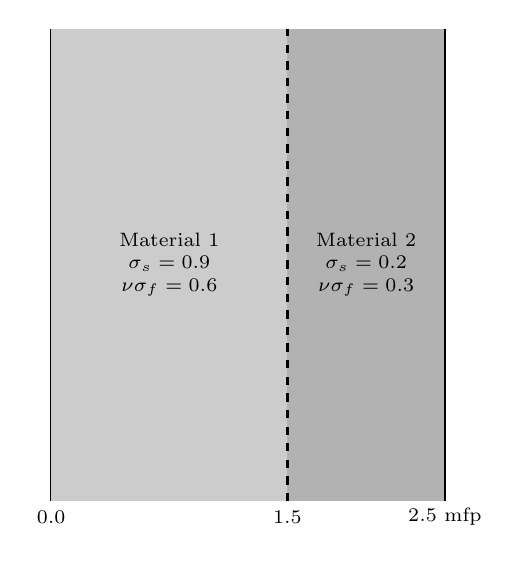
\begin{tikzpicture}[text centered]
    \begin{scope}[thick,font=\scriptsize]

    \draw [-] (-2.5,-3) -- (-2.5,3) {};
    \draw [-] (0.5,-3) -- (0.5,3) {};
    
    \draw node at (-2.5,-3.2) {$0.0$};
    \draw node at (2.5,-3.2) {$2.5$ mfp};
        \draw node at (0.5,-3.2) {$1.5$};
    
    \fill[fill=black!20] (-2.5,-3) rectangle (0.5,3);
    \fill[fill=black!30] (0.5,-3) rectangle (2.5,3);
    
    \draw [dashed] (0.5,-3) -- (0.5,3) {};
    \draw (2.5,-3) -- (2.5,3) {};
    
    \draw node [align=center] at (-1.0,0) {Material 1 \\ $\sigma_{s} = 0.9$ \\ $\nu \sigma_{f} = 0.6$};
    \draw node [align=center] at (1.5,0) {Material 2 \\ $\sigma_{s} = 0.2$ \\ $\nu \sigma_{f} = 0.3$};


    \end{scope}
\end{tikzpicture}
	\caption{Heterogeneous Multiplying Slab Benchmark Problem Domain \cite{kornreich_greens_1997}}
	\label{fig:HeteroSlabMult}
\end{figure}

\begin{figure}[!htbp]
	\centering
	\resizebox{0.75\textwidth}{!}{
	\begin{filecontents}{AlphaRQFP.dat}
x y
0.00E+00 1
1.50E-01 1.447247465
3.00E-01 1.755560563
4.50E-01 1.980425738
6.00E-01 2.125210861
7.50E-01 2.188765251
9.00E-01 2.169994135
1.05E+00 2.068765518
1.20E+00 1.885253322
1.35E+00 1.616038124
1.50E+00 1.208241837
1.60E+00 0.942444665
1.70E+00 0.777235239
1.80E+00 0.651820797
1.90E+00 0.551556358
2.00E+00 0.469075409
2.10E+00 0.399845272
2.20E+00 0.340724486
2.30E+00 0.289282031
2.40E+00 0.24323767
2.50E+00 0.198355012
\end{filecontents}

\begin{filecontents}{AlphaGFM.dat}
x    y
0    1
0.15 1.4573313
0.30 1.7677868
0.45 1.9942160
0.60 2.1400088
0.75 2.2040045
0.90 2.1851026
1.05 2.0831691
1.20 1.8983807
1.35 1.6272924
1.50 1.2166341
1.60 0.94899798
1.70 0.78264174
1.80 0.65635543
1.90 0.55539366
2.00 0.47233885
2.10 0.40262710
2.20 0.34309503
2.30 0.29129485
2.40 0.24493022
2.50 0.19900451
\end{filecontents}

\begin{tikzpicture}
\begin{axis}[
	xlabel=$x$ (MFP),
	ylabel=Scalar Flux $\phi(x)$
]
\addplot[color=red,mark=*] table {AlphaRQFP.dat};
\addlegendentry{RQFP}
\addplot[color=blue,mark=o] table {AlphaGFM.dat};
\addlegendentry{GFM}
\end{axis}
\end{tikzpicture}
	}
	\caption{Alpha-Eigenvalue Scalar Flux Results for Two-Region Multiplying Slab}
	\label{fig:TwoRegionMultiply}
\end{figure}

\clearpage
\textbf{Problem 6.1.3.3-Multiplying Five Region Fuel-Pin}:

A five region fuel-pin-like domain was modeled ($M=1000$ and $L=64$) and the alpha-eigenvalues compared to GFM for four cases. For case one and two, the fuel-pin domain consisted of five regions as seen in Figure~\ref{fig:FiveRegionProblem}, fuel, moderator, absorber, moderator, and fuel, with cross sections given in Table~\ref{table:BetzlerFive}. The leftmost fuel pin had a one mean free path width. For case one and two, the fuel fission cross section was set to $\nu \sigma_{f} = 0.3$ or $\nu \sigma_{f} = 0.7$. The alpha-eigenvalues were $\alpha = -0.3197041$ s$^{-1}$ and $\alpha = -0.0062120$ s$^{-1}$ for the $\nu \sigma_{f} = 0.3$ and $\nu \sigma_{f} = 0.7$ cases, respectively. The RQFP method eigenvalues matched the GFM-calculated alpha-eigenvalues within tolerance. Convergence of the $\nu \sigma_{f} = 0.3$ and $\nu \sigma_{f} = 0.7$ cases for the RQFP method required 30 and 27 transport sweeps, respectively. The scalar fluxes for both cases matched GFM within tolerance and are seen in Figure~\ref{fig:FiveRegionMultiply}. For cases three and four, the leftmost fuel pin width was set to 1.1. The alpha-eigenvalues for $\nu \sigma_{f} = 0.3$ and $\nu \sigma_{f} = 0.7$ were found to be -0.2932897 s$^{-1}$ and 0.0375543 s$^{-1}$, respectively. The RQFP method eigenvalues matched the GFM-calculated alpha-eigenvalues within tolerance (Table~\ref{table:FiveRegionCases}). For the supercritical case, the alpha-eigenvalue RQFP required 502 sweeps as compared to 13099 sweeps for the critical search method.

For leftmost fuel pin width of one mean free path, the $k$-effective eigenvalue of the five region fuel-pin-like was determined to be $0.42428$ and $0.98998$ for the $\nu \sigma_{f} = 0.3$ and $\nu \sigma_{f} = 0.7$ cases, respectively. For the $\nu \sigma_{f} = 0.3$ fuel pin, the RQFP method required 29 transport sweeps while the power method with fission norm update required 22 transport sweeps. For the $\nu \sigma_{f} = 0.7$ fuel pin, the RQFP method required 28 transport sweeps while the power method with fission norm update required 21 transport sweeps. For leftmost fuel pin width of 1.1 mean free paths, the $k$-effective was determined to be $0.45554$ and $1.06316$, respectively, for  $\nu \sigma_{f} = 0.3$ and $\nu \sigma_{f} = 0.7$. For the $\nu \sigma_{f} = 0.3$ fuel pin, the RQFP method required 514 transport sweeps while the power method with fission norm update required 355 transport sweeps. For the $\nu \sigma_{f} = 0.7$ fuel pin, the RQFP method required 513 transport sweeps while the power method with fission norm update required 355 transport sweeps.

\begin{figure}[!htbp]
	\centering
	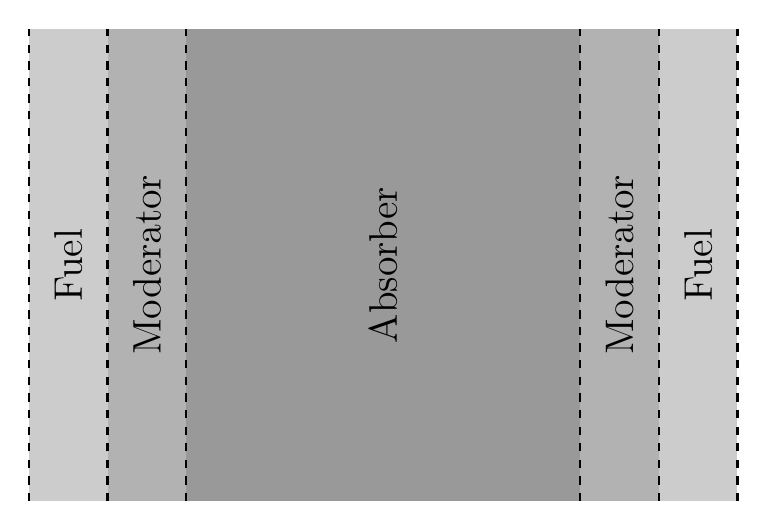
\begin{tikzpicture}
    \begin{scope}[thick,font=\scriptsize]
    
    \fill[fill=black!20] (-4.5,-3) rectangle (-3.5,3);
    \fill[fill=black!30] (-3.5,-3) rectangle (-2.5,3);
    \fill[fill=black!40] (-2.5,-3) rectangle (2.5,3);
        \fill[fill=black!30] (2.5,-3) rectangle (3.5,3);
            \fill[fill=black!20] (3.5,-3) rectangle (4.5,3);
    
    \draw [dashed] (-4.5,-3) -- (-4.5,3) {};
    \draw [dashed] (-3.5,-3) -- (-3.5,3) {};
    \draw [dashed] (-2.5,-3) -- (-2.5,3) {};
    \draw [dashed] (2.5,-3) -- (2.5,3) {};
   \draw [dashed] (3.5,-3) -- (3.5,3) {};
   \draw [dashed] (4.5,-3) -- (4.5,3) {};
   
   \draw node at (-4,0) {\Large \rotatebox[origin=c]{90}{Fuel}};
   \draw node at (-3,0) {\Large \rotatebox[origin=c]{90}{Moderator}};  
   \draw node at (-0,0) {\Large \rotatebox[origin=c]{90}{Absorber}};
   \draw node at (3,0) {\Large \rotatebox[origin=c]{90}{Moderator}};
   \draw node at (4,0) {\Large \rotatebox[origin=c]{90}{Fuel}};  

    \end{scope}
\end{tikzpicture}
	\caption{Five Region Heterogeneous Slab Benchmark Problem Domain \cite{kornreich_timeeigenvalue_2005}}
	\label{fig:FiveRegionProblem}
\end{figure}

\begin{table}[!htbp]
\centering\ra{1.3}
\caption{Comparison of RQFP- and GFM-calculated Alpha-Eigenvalues for Multiplying Five-Region Fuel-Pin}
\label{table:FiveRegionCases}
\begin{tabular}{@{}ccccc@{}}\toprule
& & \multicolumn{3}{c}{Alpha-Eigenvalue/Percent Relative Error} \\
\cmidrule{3-5} $\Delta$ & $\nu \sigma_{f}$ & RQFP & GFM & \% Relative Error \\
\midrule
%$\Delta$\\
1 & 0.3 & $-3.197041 \times 10^{-1}$ & $-3.196537 \times 10^{-2}$ & $1.58 \times 10^{-2}$ \\ 
1 & 0.7 & $-6.212026 \times 10^{-3}$ & $-6.156369 \times 10^{-3}$ & $9.041 \times 10^{-1}$ \\ 
1.1 & 0.3 & $-2.932897 \times 10^{-1}$ & $-2.93247 \times 10^{-1}$ & $1.46 \times 10 ^{-2}$ \\ 
1.1 & 0.7 & $3.75543 \times 10^{-2}$ & $3.759991 \times 10^{-2}$ & $1.213 \times 10^{-1}$ \\ 
\bottomrule
\multicolumn{5}{l}{$M = 1000$, $L = 64$, Tolerance = $10^{-12}$} \\
\end{tabular}
\end{table}

\begin{figure}[!htbp]
	\centering
	\resizebox{0.75\textwidth}{!}{
	\begin{filecontents}{Alpha03.dat}
x y
-4.500000e+00 4.988790e-01
-4.250000e+00 7.311603e-01
-4.000000e+00 8.484920e-01
-3.750000e+00 8.770258e-01
-3.500000e+00 7.985426e-01
-3.250000e+00 6.820846e-01
-3.000000e+00 5.835900e-01
-2.750000e+00 4.767421e-01
-2.500000e+00 3.391279e-01
-2.250000e+00 2.279149e-01
-2.000000e+00 1.689942e-01
-1.750000e+00 1.297957e-01
-1.500000e+00 1.022940e-01
-1.250000e+00 8.259903e-02
-1.000000e+00 6.848630e-02
-7.500000e-01 5.858579e-02
-5.000000e-01 5.203239e-02
-2.500000e-01 4.829319e-02
0.000000e+00 4.707760e-02
2.500000e-01 4.829319e-02
5.000000e-01 5.203239e-02
7.500000e-01 5.858579e-02
1.000000e+00 6.848630e-02
1.250000e+00 8.259903e-02
1.500000e+00 1.022940e-01
1.750000e+00 1.297957e-01
2.000000e+00 1.689942e-01
2.250000e+00 2.279149e-01
2.500000e+00 3.391279e-01
2.750000e+00 4.767421e-01
3.000000e+00 5.835900e-01
3.250000e+00 6.820846e-01
3.500000e+00 7.985426e-01
3.750000e+00 8.770258e-01
4.000000e+00 8.484920e-01
4.250000e+00 7.311603e-01
4.500000e+00 4.988790e-01
\end{filecontents}

\begin{filecontents}{Alpha07.dat}
-4.500000e+00 6.530922e-01
 -4.250000e+00 1.042446e+00
 -4.000000e+00 1.205673e+00
 -3.750000e+00 1.177297e+00
 -3.500000e+00 9.175721e-01
 -3.250000e+00 6.420169e-01
 -3.000000e+00 4.797641e-01
 -2.750000e+00 3.521589e-01
 -2.500000e+00 2.296407e-01
 -2.250000e+00 1.415589e-01
 -2.000000e+00 9.587206e-02
 -1.750000e+00 6.705560e-02
 -1.500000e+00 4.798165e-02
 -1.250000e+00 3.508555e-02
 -1.000000e+00 2.632529e-02
 -7.500000e-01 2.045971e-02
 -5.000000e-01 1.671996e-02
 -2.500000e-01 1.464154e-02
 0.000000e+00 1.397496e-02
 2.500000e-01 1.464154e-02
 5.000000e-01 1.671996e-02
 7.500000e-01 2.045971e-02
 1.000000e+00 2.632529e-02
 1.250000e+00 3.508555e-02
 1.500000e+00 4.798165e-02
 1.750000e+00 6.705560e-02
 2.000000e+00 9.587206e-02
 2.250000e+00 1.415589e-01
 2.500000e+00 2.296407e-01
 2.750000e+00 3.521589e-01
 3.000000e+00 4.797641e-01
 3.250000e+00 6.420169e-01
 3.500000e+00 9.175721e-01
 3.750000e+00 1.177297e+00
 4.000000e+00 1.205673e+00
 4.250000e+00 1.042446e+00
 4.500000e+00 6.530922e-01
\end{filecontents}

\begin{tikzpicture}
\begin{axis}[
	xlabel=$x$ (MFP),
	ylabel=Scalar Flux $\phi(x)$
]
\addplot[color=red,mark=*] table {Alpha03.dat};
\addlegendentry{$\nu \sigma_{f} = 0.3$}
\addplot[color=blue,mark=*] table {Alpha07.dat};
\addlegendentry{$\nu \sigma_{f} = 0.7$}
\end{axis}
\end{tikzpicture}
	}
	\caption{Case One and Two Scalar Flux Results for Five-Region Multiplying Slab-Two Cases}
	\label{fig:FiveRegionMultiply}
\end{figure}

\clearpage

\section{Multigroup Verification for Slab Geometry}

In this section, we examine the performance of the RQFP method for various multigroup-in-energy, homogeneous and heterogeneous slab benchmark problems listed in \cite{sood2003analytical}. These problems are exactly critical and problem cross sections and critical radii are given for all benchmarks. The benchmark problems provide a diverse set of nuclear system physics problem, including fast spectrum plutonium slabs, a uranium-aluminum system, highly-enriched uranium for research reactors system, and uranium-heavy water reactors.

\subsection{Multigroup Multiplying Homogeneous Slabs}

\textbf{Sood Criticality Benchmark Problem 45}: The alpha and $k$-effective eigenvalues for a two-group plutonium-239 critical slab were calculated and the RQFP method performance compared to the critical search and power methods. The plutonium-239 cross sections, listed in Table~\ref{table:TwoGroupPu239}, allowed for fission in both energy groups. Fission neutrons can be born in both energy groups with more neutrons being born in the highest energy group. The scattering cross sections of the problem do not allow for upscattering (Table~\ref{table:TwoGroupPu239_ScatterXS}).

For the critical slab width given in Table~\ref{table:SlabMG-Pu239}, the alpha-eigenvalue of the system was found to be $\alpha = -4.64633 \times 10^{-5}$ s$^{-1}$, requiring 48 transport sweeps to converge the eigenvector residual norm to a tolerance of $10^{-12}$ (Table~\ref{table:MG-Pu239-alpha}). As the problem was slightly subcritical, the critical search method did not converge to the correct eigenvalue. The $k$-effective eigenvalue was determined to be $k=0.99988$ requiring 48 transport sweeps for the RQFP method as compared to 46 transport sweeps for the power method using the fission source normalization (Table~\ref{table:MG-Pu239-k}). As the system is incredibly close to critical, the number of transport sweeps required by the RQFP method for both eigenvalues is the same. This is due to the fact that the fundamental eigenvectors are equal for both the alpha- and $k$-effective eigenvalue problems when a nuclear system is exactly critical.

\begin{table}[!htbp]
	\caption{Two-Group Plutonium-239 Problem Cross Sections (cm$^{-1}$)}
	\label{table:Pu239-TwoGroup}
	\begin{subtable}[!htbp]{1.0\textwidth}
		\centering\ra{1.3}
		\begin{tabular}{@{}cccccc@{}}\toprule
			$g$ & $\sigma_{g} $ & $\nu_{g}$ & $\sigma_{fg}$ & $\chi_{g}$ & $v_{g}$ [cm/s] \\ 
        			\midrule
			1 & 0.2208 & 3.10 & 0.0936 & 0.575 & 2.0 \\
			2 & 0.3360 & 2.93 & 0.08544 & 0.425 & 1.0 \\
			\bottomrule
		\end{tabular}
	\caption{Pu-239 Cross Sections}
	\label{table:TwoGroupPu239}
	\end{subtable}%
	\vspace{0.25cm}
	\begin{subtable}[!htbp]{1.0\textwidth}
	\centering\ra{1.3}
	\begin{tabular}{@{}ccc@{}}\toprule
	$g' \rightarrow g$ & 1 & 2 \\ 
        \midrule
	1 & 0.0792 & 0.0432 \\
	2 & 0.0 & 0.23616 \\
	\bottomrule
	\end{tabular}
	\caption{Pu-239 Scattering Block}
	\label{table:TwoGroupPu239_ScatterXS}
	\end{subtable}
\end{table}

\begin{table}[!htbp]
	\caption{Calculated Eigenvalues and Transport Sweep Comparisons for Two-Group Pu-239 Cross Sections in \cite{sood2003analytical}}
	\label{table:SlabMG-Pu239}
	\begin{subtable}[!htbp]{1.0\textwidth}
	\centering\ra{1.3}
	\begin{tabular}{@{}cccc@{}}\toprule
	& & \multicolumn{2}{c}{Transport Sweeps} \\
	\cmidrule{3-4} $r_{c}$ [cm] & Calculated $\alpha$ [s$^{-1}$] & RQFP & Critical Search\\
	\midrule
	1.795602 & $-4.64633 \times 10^{-5}$ & 48 & * \\
	\bottomrule
	\multicolumn{4}{l}{*Did Not Converge} \\
	\end{tabular}
	\caption{Alpha-Eigenvalue: Comparison of RQFP and Critical Search Transport Sweeps}
	\label{table:MG-Pu239-alpha}
	\end{subtable}%
	\vspace{0.25cm}
	\begin{subtable}[!htbp]{1.0\textwidth}
	\centering\ra{1.3}
	\begin{tabular}{@{}cccc@{}}\toprule
	& & \multicolumn{2}{c}{Transport Sweeps} \\
	\cmidrule{3-4} $r_{c}$ [cm] & Calculated $k_{\text{eff}}$ & RQFP & Power Method \\
	\midrule
	1.795602 & 0.99988 & 48 & 46 \\
	\bottomrule%	
	\multicolumn{4}{l}{$M = 500$, $L = 64$, Tolerance = $10^{-12}$} \\
	\end{tabular}
	\caption{$k$-Effective: Comparison of RQFP and Power Method Transport Sweeps}
	\label{table:MG-Pu239-k}
	\end{subtable}
\end{table}

\clearpage

\textbf{Sood Criticality Benchmark Problem 48}: The alpha and $k$-effective eigenvalues were calculated for a critical slab consisting of a uranium-235-like material. The material cross sections, seen in Table~\ref{table:TwoGroupU235}, consist of two energy groups, with fission possible in both groups. Fission neutrons can be born in both groups with a preference for the higher energy group. The material scattering cross sections (Table~\ref{table:TwoGroupU235_ScatterXS}) did not allow for upscattering.

The alpha-eigenvalue of the system was calculated to be $\alpha = -1.28364 \times 10^{-5}$ s$^{-1}$, requiring 62 transport sweeps to converge to a tolerance of $10^{-12}$ for the RQFP method. The critical search method was not able to converge (Table~\ref{table:MG-U235-alpha}). The $k$-effective eigenvalue was determined to be $k=0.99995$, requiring 62 transport sweeps for the RQFP method to converge the eigenvector. The power method required slightly fewer transport sweeps, requiring 58 transport sweeps. Similar to the plutonium-239 problem, the number of transport sweeps required by the RQFP method for both eigenvalues was the same. This was due to how close the problem was to being exactly critical.

\begin{table}[!htbp]
	\caption{Two-Group Uranium-235 Problem Cross Sections (cm$^{-1}$)}
	\label{table:U235-TwoGroup}
	\begin{subtable}[!htbp]{1.0\textwidth}
		\centering\ra{1.3}
		\begin{tabular}{@{}cccccc@{}}\toprule
			$g$ & $\sigma_{g} $ & $\nu_{g}$ & $\sigma_{fg}$ & $\chi_{g}$ & $v_{g}$ [cm/s] \\ 
        			\midrule
			1 & 0.2160 & 2.70 & 0.06192 & 0.575 & 2.0 \\
			2 & 0.3456 & 2.50 & 0.06912  & 0.425 & 1.0 \\
			\bottomrule
		\end{tabular}
	\caption{U-235 Cross Sections}
	\label{table:TwoGroupU235}
	\end{subtable}%
	\vspace{0.25cm}
	\begin{subtable}[!htbp]{1.0\textwidth}
	\centering\ra{1.3}
	\begin{tabular}{@{}ccc@{}}\toprule
	$g' \rightarrow g$ & 1 & 2 \\ 
        \midrule
	1 & 0.078240 & 0.0720  \\
	2 & 0.0 & 0.26304 \\
	\bottomrule
	\end{tabular}
	\caption{U-235 Scattering Block}
	\label{table:TwoGroupU235_ScatterXS}
	\end{subtable}
\end{table}

\clearpage

\begin{table}[!htbp]
	\caption{Calculated Eigenvalues and Transport Sweep Comparisons for Two-Group U-235 Cross Sections in \cite{sood2003analytical}}
	\label{table:SlabMG-U235}
	\begin{subtable}[!htbp]{1.0\textwidth}
	\centering\ra{1.3}
	\begin{tabular}{@{}cccc@{}}\toprule
	& & \multicolumn{2}{c}{Transport Sweeps} \\
	\cmidrule{3-4} $r_{c}$ [cm] & Calculated $\alpha$ [s$^{-1}$] & RQFP & Critical Search\\
	\midrule
	3.006375 & $-1.28364 \times 10^{-5}$ & 62 & * \\
	\bottomrule
	\multicolumn{4}{l}{*Did Not Converge} \\
	\end{tabular}
	\caption{Alpha-Eigenvalue: Comparison of RQFP and Critical Search Transport Sweeps}
	\label{table:MG-U235-alpha}
	\end{subtable}%
	\vspace{0.25cm}
	\begin{subtable}[!htbp]{1.0\textwidth}
	\centering\ra{1.3}
	\begin{tabular}{@{}cccc@{}}\toprule
	& & \multicolumn{2}{c}{Transport Sweeps} \\
	\cmidrule{3-4} $r_{c}$ [cm] & Calculated $k_{\text{eff}}$ & RQFP & Power Method\\
	\midrule
	3.006375 & 0.99995 & 62 & 58 \\
	\bottomrule%	
	\multicolumn{4}{l}{$M = 500$, $L = 64$, Tolerance = $10^{-12}$} \\
	\end{tabular}
	\caption{$k$-Effective: Comparison of RQFP and Power Method Transport Sweeps}
	\label{table:MG-U235-k}
	\end{subtable}
\end{table}

\textbf{Sood Criticality Benchmark Problem 51}: The eigenvalues of critical slab consisting of a uranium/aluminum (U/Al) mixture similar to those seen in nuclear reactor applications were calculated. The material cross sections (Table~\ref{table:TwoGroupU-Al}) consist of two energy groups with fission occurring in the lower energy ("thermal") group. All fission neutrons are born in the fast energy group. The material does not allow for upscattering (Table~\ref{table:TwoGroupU-Al_ScatterXS}) but does have a large self-scattering cross section in the lowest energy group.

The alpha-eigenvalue was calculated to be $-6.39646 \times 10^{-6}$ s$^{-1}$ and required 492 transport sweeps to converge (Table~\ref{table:MG-U-Al-alpha}). The increase in transport sweeps as compared to the plutonium and uranium problem is due to the increased scattering present in this problem. The increase in scattering, caused by the inclusion of aluminum in the cross sections, increases the number of iterations necessary to suppress higher eigenmodes in the problem. The critical search method was unable to converge the eigenvalue/eigenvector pair. The $k$-effective eigenvalue was determined to be $k=0.99985$ for the system. The RQFP method required a substantially larger number of transport sweeps as compared to power method. The RQFP method required 592 iterations as compared to 82 (Table~\ref{table:MG-U-Al-k}). The degradation of the performance of the RQFP method is due to the fact that the method converges the eigenvector as opposed to the fission source. Converging the eigenvector requires removing higher eigenmodes which require more sweeps due to the increased scattering present in the system. 

\begin{table}[!htbp]
	\caption{Two-Group U/Al Problem Cross Sections (cm$^{-1}$)}
	\label{table:U-Al}
	\begin{subtable}[!htbp]{1.0\textwidth}
		\centering\ra{1.3}
		\begin{tabular}{@{}cccccc@{}}\toprule
			$g$ & $\sigma_{g} $ & $\nu_{g}$ & $\sigma_{fg}$ & $\chi_{g}$ & $v_{g}$ [cm/s] \\ 
        			\midrule
			1 & 0.26817 & 0.0 & 0.0 & 1.0 & 2.0 \\
			2 & 1.27698 & 2.83 & 0.06070636042 & 0.0 & 1.0 \\
			\bottomrule
		\end{tabular}
	\caption{U/Al Cross Sections}
	\label{table:TwoGroupU-Al}
	\end{subtable}%
	\vspace{0.25cm}
	\begin{subtable}[!htbp]{1.0\textwidth}
	\centering\ra{1.3}
	\begin{tabular}{@{}ccc@{}}\toprule
	$g' \rightarrow g$ & 1 & 2 \\ 
        \midrule
	1 & 0.020432 & 0.247516  \\
	2 & 0.0 & 1.21313 \\
	\bottomrule
	\end{tabular}
	\caption{U/Al Scattering Block}
	\label{table:TwoGroupU-Al_ScatterXS}
	\end{subtable}
\end{table}

\begin{table}[!htbp]
	\caption{Calculated Eigenvalues and Transport Sweep Comparisons for Two-Group U/Al Mixture Cross Sections in \cite{sood2003analytical}}
	\label{table:SlabMG-U-Al}
	\begin{subtable}[!htbp]{1.0\textwidth}
	\centering\ra{1.3}
	\begin{tabular}{@{}cccc@{}}\toprule
	& & \multicolumn{2}{c}{Transport Sweeps} \\
	\cmidrule{3-4} $r_{c}$ [cm] & Calculated $\alpha$ [s$^{-1}$] & RQFP & Critical Search\\
	\midrule
	7.830630 & $-6.39646 \times 10^{-6}$ & 492 & * \\
	\bottomrule
	\multicolumn{4}{l}{*Did Not Converge} \\
	\end{tabular}
	\caption{Alpha-Eigenvalue: Comparison of RQFP and Critical Search Transport Sweeps}
	\label{table:MG-U-Al-alpha}
	\end{subtable}%
	\vspace{0.25cm}
	\begin{subtable}[!htbp]{1.0\textwidth}
	\centering\ra{1.3}
	\begin{tabular}{@{}cccc@{}}\toprule
	& & \multicolumn{2}{c}{Transport Sweeps} \\
	\cmidrule{3-4} $r_{c}$ [cm] & Calculated $k_{\text{eff}}$ & RQFP & Power Method \\
	\midrule
	7.830630 & 0.99985 & 592 & 82 \\
	\bottomrule%	
	\multicolumn{4}{l}{$M = 500$, $L = 64$, Tolerance = $10^{-12}$} \\
	\end{tabular}
	\caption{$k$-Effective: Comparison of RQFP and Power Method Transport Sweeps}
	\label{table:MG-U-Al-k}
	\end{subtable}
\end{table}

\clearpage

\textbf{Sood Criticality Benchmark Problem 54}: A highly-enriched uranium slab was modeled and the number of transport sweeps required for convergence compared between the RQFP method and standard methods. The highly-enriched uranium cross sections are similar to those found in research reactors across the world. The cross section set (Table~\ref{table:TwoGroupU93}) consists of two energy groups. Fission occurs in both energy groups with most fissions taking place in the lower energy group. However, fission neutron are only born in the highest energy ("fast") group. The cross section set allows only for downscattering of neutrons through the two energy groups with a much larger inner-group scattering cross section in the low energy group (Table~\ref{table:TwoGroupU93_ScatterXS}).

The alpha-eigenvalue of the slab was determined to be $-3.28714 \times 10^{-7}$ s$^{-1}$. The RQFP method required 1188 transport sweeps to converge the eigenvector, the increase in sweeps a product of the high amount of scattering in the system. The critical search method was not able to converge the eigenvector. The $k$-effective eigenvalue was found to be $k = 0.99999$. The RQFP method required 1188 transport sweeps to converge, similar to the alpha-eigenvalue calculation due to how close the system was to critical. The RQFP method for the $k$-effective eigenvalue required 10 times more iterations than the power method. The degradation of performance is caused by the increased scattering of the system.

\begin{table}[!htbp]
	\caption{Two-Group 93\% Enriched Uranium Problem Cross Sections (cm$^{-1}$)}
	%\label{table:U93}
	\begin{subtable}[!htbp]{1.0\textwidth}
		\centering\ra{1.3}
		\begin{tabular}{@{}cccccc@{}}\toprule
			$g$ & $\sigma_{g} $ & $\nu_{g}$ & $\sigma_{fg}$ & $\chi_{g}$ & $v_{g}$ [cm/s] \\ 
        			\midrule
			1 & 0.65696  & 2.50 & 0.0010484  & 1.0 & 2.0 \\
			2 & 2.52025 & 2.50 & 0.050632 & 0.0 & 1.0 \\
			\bottomrule
		\end{tabular}
	\caption{93\% Enriched Uranium Cross Sections}
	\label{table:TwoGroupU93}
	\end{subtable}%
	\vspace{0.25cm}
	\begin{subtable}[!htbp]{1.0\textwidth}
	\centering\ra{1.3}
	\begin{tabular}{@{}ccc@{}}\toprule
	$g' \rightarrow g$ & 1 & 2 \\ 
        \midrule
	1 & 0.62568  & 0.029227  \\
	2 & 0.0 & 2.44383  \\
	\bottomrule
	\end{tabular}
	\caption{93\% Enriched Uranium Scattering Block}
	\label{table:TwoGroupU93_ScatterXS}
	\end{subtable}
\end{table}

\begin{table}[!htbp]
	\caption{Calculated Eigenvalues and Transport Sweep Comparisons for Two-Group 93\% Enriched Uranium Mixture Cross Sections in \cite{sood2003analytical}}
	\label{table:SlabMG-U93}
	\begin{subtable}[!htbp]{1.0\textwidth}
	\centering\ra{1.3}
	\begin{tabular}{@{}cccc@{}}\toprule
	& & \multicolumn{2}{c}{Transport Sweeps} \\
	\cmidrule{3-4} $r_{c}$ [cm] & Calculated $\alpha$ [s$^{-1}$] & RQFP & Critical Search\\
	\midrule
	7.566853 & $-3.28714 \times 10^{-7}$ & 1188 & * \\
	\bottomrule
	\multicolumn{4}{l}{*Did Not Converge} \\
	\end{tabular}
	\caption{Alpha-Eigenvalue: Comparison of RQFP and Critical Search Transport Sweeps}
	\label{table:MG-U93-alpha}
	\end{subtable}%
	\vspace{0.25cm}
	\begin{subtable}[!htbp]{1.0\textwidth}
	\centering\ra{1.3}
	\begin{tabular}{@{}cccc@{}}\toprule
	& & \multicolumn{2}{c}{Transport Sweeps} \\
	\cmidrule{3-4} $r_{c}$ [cm] & Calculated $k_{\text{eff}}$ & RQFP & Power Method \\
	\midrule
	7.566853 & 0.99999 & 1188 & 98 \\
	\bottomrule%	
	\multicolumn{4}{l}{$M = 500$, $L = 64$, Tolerance = $10^{-12}$} \\
	\end{tabular}
	\caption{$k$-Effective: Comparison of RQFP and Power Method Transport Sweeps}
	\label{table:MG-U93-k}
	\end{subtable}
\end{table}

\pagebreak
\textbf{Sood Criticality Benchmark Problem 68}: To analyze the performance of the RQFP method for highly scattering systems, a two-energy group uranium/heavy water critical slab problem with cross sections given in Table~\ref{table:TwoGroupUD2O} was modeled. Fission occurs in both energy groups with all fission neutrons born in the higher energy group. However, the fission cross sections are substantially smaller than in previous systems. The system allows no upscattering but has large inner-group scattering cross sections for both groups (Table~\ref{table:TwoGroupUD2O_ScatterXS}). The critical radius of the slab is much larger than previous problems, due to the small fission cross sections and highly scattering nature of the problem.

For the critical radius listed in Table~\ref{table:MG-UD2O-alpha}, the alpha-eigenvalue was determined to be $-6.93314 \times 10^{-7}$ s$^{-1}$. The RQFP method required 451136 transport sweeps for convergence, a substantial increase as compared to the previous problems (Table~\ref{table:MG-UD2O-alpha}). The critical search method was unable to converge the eigenvalue and eigenvector pair. The $k$-effective eigenvalue was determined to be $k = 0.99887$. The RQFP method required 451136 transport sweeps, performing far worse than the power method which only required 52964 transport sweeps to converge (Table~\ref{table:MG-UD2O-k}). The sensitivity of the RQFP method to scattering cross sections implies the convergence of the fixed point iteration is determined by the scattering cross sections.

\begin{table}[!htbp]
	\caption{Two-Group U-D$_{2}$O Problem Cross Sections (cm$^{-1}$)}
	%\label{table:U93}
	\begin{subtable}[!htbp]{1.0\textwidth}
		\centering\ra{1.3}
		\begin{tabular}{@{}cccccc@{}}\toprule
			$g$ & $\sigma_{g} $ & $\nu_{g}$ & $\sigma_{fg}$ & $\chi_{g}$ & $v_{g}$ [cm/s] \\ 
        			\midrule
			1 & 0.33588  & 2.50 & 0.002817 & 1.0 & 2.0 \\
			2 & 0.54628  & 2.50 & 0.097 & 0.0 & 1.0 \\
			\bottomrule
		\end{tabular}
	\caption{U-D$_{2}$O Cross Sections}
	\label{table:TwoGroupUD2O}
	\end{subtable}%
	\vspace{0.25cm}
	\begin{subtable}[!htbp]{1.0\textwidth}
	\centering\ra{1.3}
	\begin{tabular}{@{}ccc@{}}\toprule
	$g' \rightarrow g$ & 1 & 2 \\ 
        \midrule
	1 & 0.31980   & 0.004555   \\
	2 & 0.0 & 0.42410  \\
	\bottomrule
	\end{tabular}
	\caption{U-D$_{2}$O Scattering Block}
	\label{table:TwoGroupUD2O_ScatterXS}
	\end{subtable}
\end{table}

\begin{table}[!htbp]
	\caption{Calculated Eigenvalues and Transport Sweep Comparisons for Two-Group U-D$_{2}$O Cross Sections in \cite{sood2003analytical}}
	\label{table:SlabMG-UD2O}
	\begin{subtable}[!htbp]{1.0\textwidth}
	\centering\ra{1.3}
	\begin{tabular}{@{}cccc@{}}\toprule
	& & \multicolumn{2}{c}{Transport Sweeps} \\
	\cmidrule{3-4} $r_{c}$ [cm] & Calculated $\alpha$ [s$^{-1}$] & RQFP & Critical Search\\
	\midrule
	846.632726 & $-6.93314 \times 10^{-7}$ & 451140 & * \\
	\bottomrule
	\multicolumn{4}{l}{*Did Not Converge} \\
	\end{tabular}
	\caption{Alpha-Eigenvalue: Comparison of RQFP and Critical Search Transport Sweeps}
	\label{table:MG-UD2O-alpha}
	\end{subtable}%
	\vspace{0.25cm}
	\begin{subtable}[!htbp]{1.0\textwidth}
	\centering\ra{1.3}
	\begin{tabular}{@{}cccc@{}}\toprule
	& & \multicolumn{2}{c}{Transport Sweeps} \\
	\cmidrule{3-4} $r_{c}$ [cm] & Calculated $k_{\text{eff}}$ & RQFP & Power Method \\
	\midrule
	846.632726 & 0.99887 & 451136 & 52964 \\
	\bottomrule%	
	\multicolumn{4}{l}{$M = 2000$, $L = 64$, Tolerance = $10^{-12}$} \\
	\end{tabular}
	\caption{$k$-Effective: Comparison of RQFP and Power Method Transport Sweeps}
	\label{table:MG-UD2O-k}
	\end{subtable}
\end{table}

\clearpage
\subsection{Multigroup Reflected Slabs}

Two water-reflected research reactor-like slab problems were considered. For the cross section sets shown in Table~\ref{table:Ub-H2O} and Table ~\ref{table:Uc}, fissile slabs were reflected by a water reflector on the right side of the slab that made the problem exactly critical. The two-group cross section sets allowed for upscattering. The fissile slab width along with slab and reflector width are listed in Table~\ref{table:SlabMG-RRH2O}.

The reflected slab problems were found to be slightly subcritical (Table~\ref{table:MG-RRH2O-alpha}). Using the Rayleigh Quotient Fixed Point method for the alpha-eigenvalue, the alpha-eigenvalue and eigenvector were determined in 2042 and 3192 transport sweeps. Due to the large amounts of scattering in the reflector, the convergence rate of the method was slowed and required many more transport sweeps as compared to problems with less scattering. Attempting to calculate the alpha-eigenvalue with the critical search method was unsuccessful due to the negative alpha-eigenvalue. Despite the problems only being slightly subcritical, the critical search method was unable to converge the problems.

For the $k$-effective eigenvalue, the Rayleigh Quotient Fixed Point method underperformed the power method with fission source update dramatically (Table~\ref{table:MG-RRH2O-k}). The RQFP method required 20-30 times the number of iterations as compared to the default method. Since the reflected slabs were only slightly subcritical, the number of transport sweeps required to converge the alpha- and $k$-effective eigenvalues were similar. With convergence of the fixed point methods determined by the scattering present in the problems, the scattering in the water reflector slowed down convergence dramatically. With the fission source update only concerned with fissile regions of the problem, convergence was achieved faster as the water reflector had less of an impact on the convergence rate.

\begin{table}[!htbp]
	\caption{Two-Group Research Reactor (b) and Water Reflector Problem Cross Sections (cm$^{-1}$)}
	\label{table:Ub-H2O}
	\begin{subtable}[!htbp]{1.0\textwidth}
		\centering\ra{1.3}
		\begin{tabular}{@{}cccccc@{}}\toprule
			$g$ & $\sigma_{g} $ & $\nu_{g}$ & $\sigma_{fg}$ & $\chi_{g}$ & $v_{g}$ [cm/s] \\ 
        			\midrule
			1 & 0.88721  & 2.50 & 0.000836 & 1.0 & 2.0 \\
			2 & 2.9727  & 2.50 & 0.029564 & 0.0 & 1.0 \\
			\bottomrule
		\end{tabular}
	\caption{Research Reactor (b) Cross Sections}
	\label{table:TwoGroupUb-H2O}
	\end{subtable}%
	\vspace{0.25cm}
	\begin{subtable}[!htbp]{1.0\textwidth}
	\centering\ra{1.3}
	\begin{tabular}{@{}ccc@{}}\toprule
	$g' \rightarrow g$ & 1 & 2 \\ 
        \midrule
	1 & 0.83892 & 0.04635   \\
	2 & 0.000767 & 2.9183  \\
	\bottomrule
	\end{tabular}
	\caption{Research Reactor (b) Scattering Block}
	\label{table:TwoGroupUb_ScatterXS}
	\end{subtable}%
	\vspace{0.25cm}
	\begin{subtable}[!htbp]{1.0\textwidth}
		\centering\ra{1.3}
		\begin{tabular}{@{}cccccc@{}}\toprule
			$g$ & $\sigma_{g} $ & $\nu_{g}$ & $\sigma_{fg}$ & $\chi_{g}$ & $v_{g}$ [cm/s] \\ 
        			\midrule
			1 & 0.88798  & 0.0 & 0.0 & 0.0 & 2.0 \\
			2 & 2.9865  & 0.0 & 0.0 & 0.0 & 1.0 \\
			\bottomrule
		\end{tabular}
	\caption{H$_{2}$O Cross Sections}
	\label{table:TwoGroupH2O}
	\end{subtable}%
	\vspace{0.25cm}
	\begin{subtable}[!htbp]{1.0\textwidth}
	\centering\ra{1.3}
	\begin{tabular}{@{}ccc@{}}\toprule
	$g' \rightarrow g$ & 1 & 2 \\ 
        \midrule
	1 & 0.83975 & 0.04749   \\
	2 & 0.000336 & 2.9676  \\
	\bottomrule
	\end{tabular}
	\caption{H$_{2}$O Scattering Block}
	\label{table:TwoGroupH2O_ScatterXS}
	\end{subtable}
\end{table}

\begin{table}[!htbp]
	\caption{Two-Group Research Reactor (c) Problem Cross Sections (cm$^{-1}$)}
	\label{table:Uc}
	\begin{subtable}[!htbp]{1.0\textwidth}
		\centering\ra{1.3}
		\begin{tabular}{@{}cccccc@{}}\toprule
			$g$ & $\sigma_{g} $ & $\nu_{g}$ & $\sigma_{fg}$ & $\chi_{g}$ & $v_{g}$ [cm/s] \\ 
        			\midrule
			1 & 0.88655  & 2.50 & 0.001648 & 1.0 & 2.0 \\
			2 & 2.9628  & 2.50 & 0.057296 & 0.0 & 1.0 \\
			\bottomrule
		\end{tabular}
	\caption{Research Reactor (c) Cross Sections}
	\label{table:TwoGroupUb}
	\end{subtable}%
	\vspace{0.25cm}
	\begin{subtable}[!htbp]{1.0\textwidth}
	\centering\ra{1.3}
	\begin{tabular}{@{}ccc@{}}\toprule
	$g' \rightarrow g$ & 1 & 2 \\ 
        \midrule
	1 & 0.83807 & 0.04536   \\
	2 & 0.00116 & 2.8751  \\
	\bottomrule
	\end{tabular}
	\caption{Research Reactor (c) Scattering Block}
	\label{table:TwoGroupUc_ScatterXS}
	\end{subtable}%
\end{table}

\begin{table}[!htbp]
	\caption{Calculated Eigenvalues and Transport Sweep Comparisons for H$_{2}$O-Reflected Research Reactor Cross Sections in \cite{sood2003analytical}}
	\label{table:SlabMG-RRH2O}
	\begin{subtable}[!htbp]{1.0\textwidth}
	\centering\ra{1.3}
	\resizebox{1.00\textwidth}{!}{
	\begin{tabular}{@{}cccccc@{}}\toprule
	& & & & \multicolumn{2}{c}{Transport Sweeps} \\
	\cmidrule{5-6} Cross Section Set & $r_{c}$ [cm] & $r_{c} + r_{\text{refl}}$ [cm] & Calculated $\alpha$ [s$^{-1}$] & RQFP & Critical Search\\
	\midrule
	 Research Reactor (b)/H$_{2}$O & 6.696802 & 7.822954 &  $-1.10466 \times 10^{-7}$ & 2042 & * \\
 	 Research Reactor (c)/H$_{2}$O & 4.863392 & 10.494149 & $-5.92658 \times 10^{-9}$ & 3192 & * \\
	\bottomrule
	\multicolumn{6}{l}{*Did Not Converge} \\
	\end{tabular}}
	\caption{Alpha-Eigenvalue: Comparison of RQFP and Critical Search Transport Sweeps}
	\label{table:MG-RRH2O-alpha}
	\end{subtable}%
	\vspace{0.25cm}
	\begin{subtable}[!htbp]{1.0\textwidth}
	\centering\ra{1.3}
	\resizebox{1.00\textwidth}{!}{
	\begin{tabular}{@{}cccccc@{}}\toprule
	& & & & \multicolumn{2}{c}{Transport Sweeps} \\
\cmidrule{5-6} Cross Section Set & $r_{c}$ [cm] & $r_{c} + r_{\text{refl}}$ [cm] & Calculated $k_{\text{eff}}$ & RQFP & Power Method\\
	\midrule
	 Research Reactor (b)/H$_{2}$O & 6.696802 & 7.822954 & 0.99999 & 2038 & 112 \\
  	 Research Reactor (c)/H$_{2}$O & 4.863392 & 10.494149 & 0.99999 & 3280 & 94 \\
	\bottomrule%	
	\multicolumn{6}{l}{$M = 2000$, $L = 64$, Tolerance = $10^{-12}$} \\
	\end{tabular}}
	\caption{$k$-Effective: Comparison of RQFP and Power Method Transport Sweeps}
	\label{table:MG-RRH2O-k}
	\end{subtable}
\end{table}

\clearpage
\section{One-Speed Verification for Spherical Geometry}

In certain circumstances, alpha-eigenvalue results for slab geometry also apply to spherical geometry problems. This slab-sphere equivalence holds for isotropically scattering heterogeneous media where the total cross section is equal for all regions \cite{davison1957neutron}. More generally, a convenient property of spherically symmetric systems is that if the mean free path in the system is independent of position and scattering is isotropic, then the determination of the spherically symmetric neutron distribution of these systems is reduced to the determination of these distributions in certain systems with plane symmetries. Thus, for all homogeneous slab and symmetric heterogeneous slab systems where each region has the same total cross section, it follows that there exists a spherical equivalent for the problems studied in the previous sections. Specifically, it can be shown that the second eigenvalue of a slab system is identical to the fundamental eigenvalue for the equivalent sphere. In this section, we examine the performance of the RQFP method for one-dimensional spherical problems which are equivalent to the slab problems from before. We verify the correctness of the method for this subset of problems and compare its performance to the critical search and power methods.

\subsection{Non-Multiplying Homogeneous Spheres}

To verify the correctness of the RQFP method for one-dimensional spherical geometry, four non-multiplying homogeneous slab problems in \cite{kornreich_greens_1997} with a second eigenvalue listed were modeled as equivalent spherical problems with radii of $\Delta/2$ mfp \cite{}.The dominant alpha-eigenvalue of the equivalent spherical systems is the second eigenvalue of the slab problems. The calculated alpha-eigenvalues were then compared to the GFM-calculated eigenvalues. The purely homogeneous scattering spheres used the cross sections listed in Table~\ref{table:Betzler}. For all problems, the percent relative error between the RQFP- and GFM-calculated eigenvalues was less than 0.005 \% (Table~\ref{table:CompHomogScattSphere}) for diamond differencing discretization ($M=500$) and an S$_{64}$ discrete ordinates quadrature in angle ($L=64$). As the radius of the spheres increases, the system approaches the critical state and the alpha-eigenvalue approaches zero. However, as there is no fissile material, the eigenvalue can never reach zero.

\begin{table*}[!htbp]
\centering\ra{1.3}
\caption{Comparison of RQFP- and GFM-Calculated Alpha-Eigenvalues for a Homogeneous Scattering Sphere}
\label{table:CompHomogScattSphere}
\begin{tabular}{@{}cccc@{}}\toprule
& \multicolumn{3}{c}{Alpha-Eigenvalue/Percent Relative Error} \\
\cmidrule{2-4} $\Delta$ & RQFP & GFM & \% Relative Error \\
\midrule
5 & $-3.41177 \times 10^{-1}$ & $-3.41216 \times 10^{-1}$ & 0.0114 \\ 
10 & $-1.02973 \times 10^{-1}$ & $-1.02978 \times 10^{-1}$ & 0.0049 \\ 
20 & $-2.88443 \times 10^{-2}$ & $-2.88447 \times 10^{-2}$ & 0.0014 \\ 
25 & $-1.89226 \times 10^{-2}$ & $-1.89228 \times 10^{-2}$ & 0.0011 \\ 
\bottomrule
\multicolumn{4}{l}{$M = 500$, $L = 64$, Tolerance = $10^{-12}$} \\
\end{tabular}
\end{table*}

\subsection{Multiplying Homogeneous Spheres}

For homogeneous slab problems with multiplication (Cross sections-Table~\ref{table:Betzler2}), the equivalent spherical problems were modeled and the performance and correctness of the RQFP methods for alpha- and $k$-effective eigenvalue calculations were examined.

To verify the correctness of the RQFP method for alpha-eigenvalue problems, the RQFP-calculated eigenvalues were compared to the GFM-calculated eigenvalues listed in \cite{kornreich_greens_1997}. The problems were modeled using diamond differencing ($M=500$) and an S$_{64}$ discrete ordinates quadrature in angle ($L=64$). For spherical problems with diameters ranging from three to 50 mean free paths, it was found that the eigenvalues agreed within 0.02\% relative error (Table~\ref{table:CompHomogMultSphere}). Alpha-eigenvalue agreement increased as the spherical system became larger. In all cases, the RQFP method was able to correctly determine the criticality of the system, even for systems that were slightly subcritical or supercritical.

The performance of the RQFP method for alpha-eigenvalue problems was compared to the critical search method. The number of transport sweeps required to converge the eigenvector norm residual to a tolerance of $10^{-12}$ for various spherical radii is seen in Table~\ref{table:CompMultSweepsSphere}. For problem that were subcritical ($\Delta = 3 - 7$ mfp), the RQFP method was able to converge to the correct eigenvalue while the critical search method was not able to converge the problem. As problems became increasingly supercritical, the number of transport sweeps required to converge increased for both the RQFP and critical search methods. This is due to the fact that as the systems become larger, neutrons can survive longer before being absorbed or leaking out of the system. These longer lived neutrons cause the increase in the alpha-eigenvalue but more transport sweeps are required before reaching the fundamental mode of the angular flux. For the supercritical cases, the critical search method was able to correctly determine the eigenvalue of the spherical systems. However, in all cases, the number of transport sweeps required by the RQFP method was approximately 20-40 times less than the critical search method.

The RQFP method was compared to the power method with a fission norm update for the $k$-effective eigenvalue. In all cases, the power method performed better than the RQFP method. The number of transport sweeps necessary to converge was similar to subcritical and slightly supercritical problems for both methods. However, as the problems became more supercritical, the RQFP method's performance deteriorated (Table~\ref{table:CompMultSweepsKSphere}).

\begin{table*}[!htbp]
\centering\ra{1.3}
\caption{Comparison of RQFP- and GFM-Calculated Alpha-Eigenvalues for a Homogeneous Scattering Multiplying Sphere}
\label{table:CompHomogMultSphere}
\begin{tabular}{@{}cccc@{}}\toprule
& \multicolumn{3}{c}{Alpha-Eigenvalue/Percent Relative Error} \\
\cmidrule{2-4} $\Delta$ & RQFP & GFM & \% Relative Error \\
\midrule
3 & $-5.68218 \times 10^{-1}$ & $-5.6833 \times 10^{-1}$ & 0.0197 \\ 
4 & $-3.00486 \times 10^{-1}$ & $-3.0054 \times 10^{-1}$ & 0.0180 \\ 
5 & $ -1.60321 \times 10^{-1}$ & $-1.6035 \times 10^{-1}$ & 0.0181 \\ 
6 & $ -7.72739 \times 10^{-2}$ & $-7.7292 \times 10^{-2}$ & 0.0234 \\ 
7 & $-2.38450 \times 10^{-2}$ & $-2.3857 \times 10^{-2}$ & 0.0503 \\ 
8 & $1.26235 \times 10^{-2}$ & $1.2616 \times 10^{-2}$ & 0.0594 \\ 
9 & $ 3.86541 \times 10^{-2}$ & $3.8649 \times 10^{-2}$ & 0.0132 \\ 
10 & $5.78980 \times 10^{-2}$ & $5.7894 \times 10^{-2}$ & 0.0069 \\ 
15 & $1.06258 \times 10^{-1}$ & $1.0626 \times 10^{-1}$ & 0.0019 \\ 
20 & $1.24512 \times 10^{-1}$ & $1.2451 \times 10^{-1}$ &  0.0016 \\ 
30 & $1.38248 \times 10^{-1}$ & $1.3825 \times 10^{-1}$ &  0.0014 \\ 
40 & $1.43262 \times 10^{-1}$ & $1.4326 \times 10^{-1}$ &  0.0014 \\ 
50 & $1.45638 \times 10^{-1}$ & $1.4564 \times 10^{-1}$ &  0.0014 \\ 
\bottomrule
\multicolumn{4}{l}{$M = 500$, $L = 64$, Tolerance = $10^{-12}$} \\
\end{tabular}
\end{table*}

\begin{table}[!htbp]
	\caption{Transport Sweep Comparisons for Homogeneous Multiplying Spheres}
	\begin{subtable}[!htbp]{1.0\textwidth}
	\centering\ra{1.3}
	\begin{tabular}{@{}cccccc@{}}\toprule
	& \multicolumn{2}{c}{Transport Sweeps} & & \multicolumn{2}{c}{Transport Sweeps} \\
	\cmidrule{2-3} \cmidrule{5-6} $\Delta$ & RQFP & Critical Search \quad &  \Delta & RQFP & Critical Search\\
	\midrule
3 & 46 & * & 10 & 128 & 29645 \\
4 & 46 & * & 15 & 227 & 61303 \\
5 & 52 & * & 20 & 357 & 84353 \\
6 & 67 & * & 30 & 707 & 100433 \\
7 & 81 & * & 40 & 1176 & 99135 \\
8 & 96 & 10865 & 50 & 1761 & 97037 \\
9 & 111 & 21555 & & & \\ 
	\bottomrule
	\multicolumn{6}{l}{*Did Not Converge} \\
	\end{tabular}
	\caption{Alpha-Eigenvalue: Comparison of RQFP and Critical Search Sweeps}
	\label{table:CompMultSweepsSphere}
	\end{subtable}%
	\vspace{0.25cm}
	\begin{subtable}[!htbp]{1.0\textwidth}
	\centering\ra{1.3}
	\begin{tabular}{@{}cccccc@{}}\toprule
	& \multicolumn{2}{c}{Transport Sweeps} & & \multicolumn{2}{c}{Transport Sweeps} \\
	\cmidrule{2-3} \cmidrule{5-6} $\Delta$ & RQFP & Power Method \quad &  \Delta & RQFP & Power Method\\
	\midrule
3 & 49 & 43 & 10 & 127 & 62 \\ 
4 & 57 & 47 & 15 & 214 & 79 \\
5 & 66 & 49 & 20 & 329 & 103 \\
6 & 76 & 52 & 30 & 636 & 167 \\ 
7 & 87 & 54 & 40 & 1049 & 253 \\ 
8 & 99 & 56 & 50 & 1562 & 360 \\ 
9 & 113 & 59 &  &  &  \\ 
	\bottomrule
	\multicolumn{6}{l}{$M = 500$, $L = 64$, Tolerance = $10^{-12}$} \\
	\end{tabular}
	\caption{$k$-Effective: Comparison of RQFP and Power Method Transport Sweeps}
	\label{table:CompMultSweepsKSphere}
	\end{subtable}
\end{table}

%\begin{table*}[t]
%\centering\ra{1.3}
%\caption{Alpha-Eigenvalue: Comparison of RQFP and Critical Search Sweeps for Homogeneous Multiplying Spheres}
%\label{table:CompMultSweepSpheres}
%\begin{tabular}{@{}cccccc@{}}\toprule
%& \multicolumn{2}{c}{Transport Sweeps} & & \multicolumn{2}{c}{Transport Sweeps} \\
%\cmidrule{2-3} \cmidrule{5-6} $\Delta$ & RQFP & Critical Search \quad &  \Delta & RQFP & Critical Search\\
%\midrule
%%$\Delta$\\
%%8 & 98 & 10865 & 20 & 364 & 84353\\ 
%%9 & 113 & 21555 & 30 & 722 & 100433 \\
%%10 & 130 & 29645 & 40 & 1201 & 99135 \\
%%15 & 232 & 61303 & 50 & 1799 & 97037 \\
%3 & x & * & 10 & 130 & 29645 \\
%4 & x & * & 15 & 232 & 61303 \\
%5 & x & * & 20 & 364 & 84353 \\
%6 & x & * & 30 & 722 & 100433 \\
%7 & x & * & 40 & 1201 & 99135 \\
%8 & 98 & 10865 & 50 & 1799 & 97037 \\
%9 & 113 & 21555 & & & \\ 
%\bottomrule
%\multicolumn{6}{l}{$M = 500$, $L = 64$, Tolerance = $10^{-12}$} \\
%\end{tabular}
%\end{table*}
%
%\begin{table*}[t]
%\centering\ra{1.3}
%\caption{$k$-Effective Eigenvalue: Comparison of RQFP and Power Method with Fission Norm Sweeps for Homogeneous Multiplying Spheres}
%\label{table:CompMultSweepSpheresK}
%\begin{tabular}{@{}cccccc@{}}\toprule
%& \multicolumn{2}{c}{Transport Sweeps} & & \multicolumn{2}{c}{Transport Sweeps} \\
%\cmidrule{2-3} \cmidrule{5-6} $\Delta$ & RQFP & Power Method \quad &  \Delta & RQFP & Power Method\\
%\midrule
%%$\Delta$\\
%3 & 49 & 43 & 10 & 127 & 62 \\ 
%4 & 57 & 47 & 15 & 214 & 79 \\
%5 & 66 & 49 & 20 & 329 & 103 \\
%6 & 76 & 52 & 30 & 636 & 167 \\ 
%7 & 87 & 54 & 40 & 1049 & 253 \\ 
%8 & 99 & 56 & 50 & 1562 & 360 \\ 
%9 & 113 & 59 &  &  &  \\ 
%\bottomrule
%\multicolumn{6}{l}{$M = 500$, $L = 64$, Tolerance = $10^{-12}$} \\
%\end{tabular}
%\end{table*}

\clearpage

\subsection{Multiplying Homogeneous Spheres with Anisotropic Scattering}

Three exactly critical multiplying homogeneous spheres with anisotropic scattering were modeled to determine the impacts of higher scattering order cross sections on the performance of the RQFP methods. Three sets of uranium-heavy water cross sections sets (Table~\ref{table:SoodUD2OAniso}) were examined, each with different anisotropic scattering cross section orders. In particular, cross section set U-D$_{2}$O (c) had a negative anisotropic scattering cross section. The critical radii for the three problems are listed in Table~\ref{table:AnisoSphere}. These problems were modeled using the diamond differencing scheme in space (500 cells), and S$_{64}$ discrete ordinate angular quadrature.

For alpha-eigenvalue problems, the RQFP method calculated alpha-eigenvalues that were within $10^{-7}$ of the true alpha-eigenvalue of zero. For two cases, U-D$_{2}$O (a) and U-D$_{2}$O (b), the problems were slightly supercritical, while for U-D$_{2}$O (c) the problem was subcritical. For the two supercritical cases, both the RQFP and critical search methods were able to converge to the same eigenvalue. The RQFP method required approximately half the transport sweeps as compared to the critical search method (Table~\ref{table:AnisoSphereAlpha}). For the subcritical case, the critical search method could not converge to the correct eigenvalue as the problem was too close to critical and subcritical. For the RQFP method, the number of transport sweeps required to converge the case with a negative anisotropic scattering cross section increased by a factor of 1.5 as compared to non-negative anisotropic cross sections. This suggests the negative anisotropic cross section can impact the rate of convergence.

For $k$-effective eigenvalue problems, the RQFP method calculated $k$-effective eigenvalues were within $10^{-7}$ of the true value of $k_{\text{eff}}=1.00000$. In all three cases, the RQFP method required approximately double the iterations as compared to the power method with fission norm update (Table~\ref{table:AnisoSpherek}). Similar to the alpha-eigenvalue problems, the inclusion of a negative anisotropic scattering cross section increased the number of transport sweeps necessary to converge to a tolerance of $10^{-12}$.

\begin{table}[!htbp]
	\caption{Uranium-Heavy Water Cross Sections with Anisotropic Scattering for Critical Sphere Problems (cm$^{-1}$) \cite{sood2003analytical}}
	\label{table:SoodUD2OAniso}
	\centering\ra{1.3}
    \begin{tabular}{*6c}
        \toprule
	Cross Section Set & $\sigma$ & $\nu \sigma_{f}$ & $\sigma_{s0}$  & $\sigma_{s1}$ & $v$ [cm/s] \\ 
        \midrule
	U-D$_{2}$O (a)  & 0.54628 & 0.098788237268 & 0.464338 & 0.056312624 & 1 \\
	U-D$_{2}$O (b)  & 0.54628 & 0.100574846008 & 0.464338 & 0.112982569 & 1 \\
	U-D$_{2}$O (c)  & 0.54628 & 0.0926709392 & 0.464338 & -0.27850447 & 1 \\
        \bottomrule
    \end{tabular}
\end{table}

\begin{table}[!htbp]
	\caption{Calculated Eigenvalues and Transport Sweep Comparisons for Critical Sphere Problems with Anisotropic Scattering in \cite{sood2003analytical}}
	\label{table:AnisoSphere}
	\begin{subtable}[!htbp]{1.0\textwidth}
	\centering\ra{1.3}
	\begin{tabular}{@{}ccccc@{}}\toprule
	& & & \multicolumn{2}{c}{Transport Sweeps} \\
	\cmidrule{4-5} Cross Section Set & r$_{c}$ [cm] & Calculated $\alpha$ [s$^{-1}$] & RQFP & Critical Search\\
	\midrule
	U-D$_{2}$O (a) & 18.30563081 & $3.165772 \times 10^{-7}$ & 299 & 585 \\
	U-D$_{2}$O (b) & 18.30563081 & $3.930857 \times 10^{-7}$ & 270 & 541\\
	U-D$_{2}$O (c) & 18.30563081 & $ -6.613381 \times 10^{-7}$ & 456 & *\\
	\bottomrule
	\multicolumn{5}{l}{*Did Not Converge} \\
	\end{tabular}
	\caption{Alpha-Eigenvalue: Comparison of RQFP and Critical Search Transport Sweeps}
	\label{table:AnisoSphereAlpha}
	\end{subtable}%
	\vspace{0.25cm}
	\begin{subtable}[!htbp]{1.0\textwidth}
	\centering\ra{1.3}
	\begin{tabular}{@{}ccccc@{}}\toprule
	& & \multicolumn{2}{c}{Transport Sweeps} \\
	\cmidrule{4-5} Cross Section Set & r$_{c}$ [cm] & Reference $k_{\text{eff}}$ & RQFP & Power Method \\
	\midrule
	U-D$_{2}$O (a) & 18.30563081 & 1.000003 & 301 & 118 \\
	U-D$_{2}$O (b) & 18.30563081 & 1.000003 & 273 & 106 \\
	U-D$_{2}$O (c) & 18.30563081 & 0.999993 & 456 & 207 \\
	\bottomrule
	\multicolumn{5}{l}{$M = 500$, $L = 64$, Tolerance = $10^{-12}$} \\
	\end{tabular}
	\caption{$k$-Effective: Comparison of RQFP and Power Method Transport Sweeps}
	\label{table:AnisoSpherek}
	\end{subtable}
\end{table}

\clearpage

\subsection{A Spherical Shell Problem}

To verify the correctness of the alpha-eigenvalue RQFP method, two spherical shell problems were modeled and the calculated alpha-eigenvalues compared to the GFM-calculated value in \cite{kornreich_greens_1997}. For any symmetric heterogeneous slab problem, an equivalent spherical shell problem can be modeled. As before, the second eigenvalue of the heterogeneous slab problem is the dominant eigenvalue of the spherical shell problem. Using the five-region fuel pin from Figure~\ref{fig:FiveRegionProblem} with the right fuel pin width set to one mean free path, an equivalent spherical problem shown in Figure~\ref{fig:FiveRegionSphereProblem} was modeled. For this particular problem, the width of each material section remained the same as in the five region slab case. Cross sections for the three materials were the same as the slab geometry problem (Table~\ref{table:BetzlerFive}). Similar to the five region slab problem, two cases were examined where $\nu \sigma_{f} = 0.3$ and $0.7$.

The RQFP- and GFM-calculated alpha-eigenvalues are listed in Table~\ref{table:FiveRegionCasesSphere}. For the $\nu \sigma_{f} = 0.3$ case, the alpha-eigenvalues matched within 0.5\%. For the $\nu \sigma_{f} = 0.7 $ case, agreement was within 2.2\%. The higher discrepancy in the eigenvalue was most likely due to the neutron angular redistribution of spherical geometry as compared to Cartesian coordinates in ARDRA. The GFM-calculated alpha-eigenvalue uses analytic Green's Functions and then determines the eigenvalues numerical through a search process and does not discretize the underlying integro-differential equation like ARDRA.

\begin{figure}[!htbp]
	\centering
	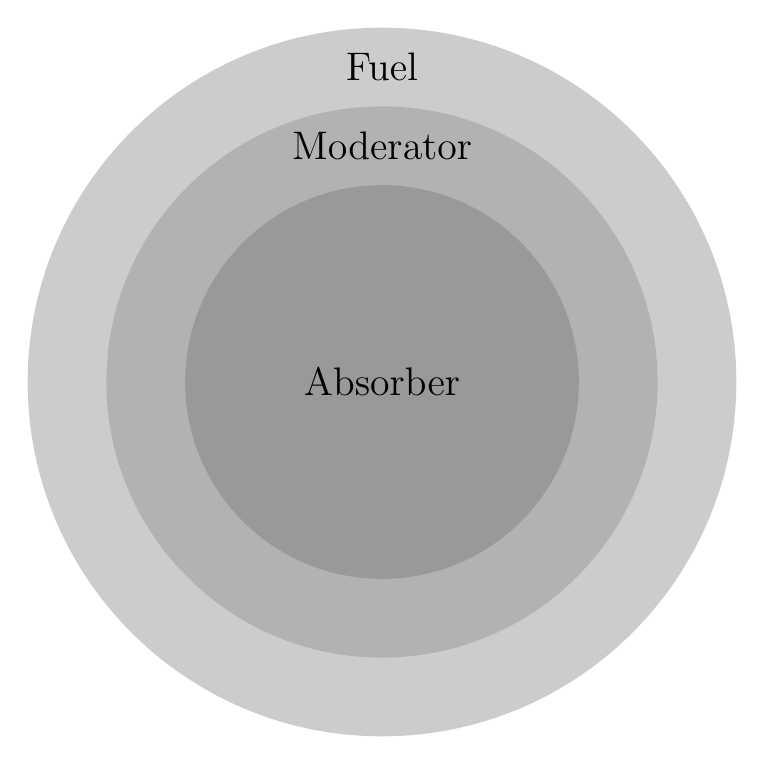
\begin{tikzpicture}
    \begin{scope}[thick,font=\scriptsize]
   
    \fill[fill=black!20] circle (4.5);
    \fill[fill=black!30] circle (3.5);    
    \fill[fill=black!40] circle (2.5);    
    
    \draw node at (0,0) {\Large \rotatebox[origin=c]{0}{Absorber}};
    \draw node at (0,3) {\Large \rotatebox[origin=c]{0}{Moderator}};  
    \draw node at (0,4) {\Large \rotatebox[origin=c]{0}{Fuel}};  
%   \draw node at (-4,0) {\Large \rotatebox[origin=c]{90}{Fuel}};
%   \draw node at (-3,0) {\Large \rotatebox[origin=c]{90}{Moderator}};  
%   \draw node at (-0,0) {\Large \rotatebox[origin=c]{90}{Absorber}};
%   \draw node at (3,0) {\Large \rotatebox[origin=c]{90}{Moderator}};
%   \draw node at (4,0) {\Large \rotatebox[origin=c]{90}{Fuel}};  

    \end{scope}
\end{tikzpicture}
	\caption{Five Region Fuel Pin Spherical Equivalent \cite{kornreich_timeeigenvalue_2005}}
	\label{fig:FiveRegionSphereProblem}
\end{figure}

\begin{table*}[!htbp]
\centering\ra{1.3}
\caption{Comparison of RQFP- and GFM-calculated Alpha-Eigenvalues for a Three Region Multiplying Sphere}
\label{table:FiveRegionCasesSphere}
\begin{tabular}{@{}cccc@{}}\toprule
& \multicolumn{3}{c}{Alpha-Eigenvalue/Percent Relative Error} \\
\cmidrule{2-4} $\nu \sigma_{f}$ & RQFP & GFM & \% Relative Error \\
\midrule
%$\Delta$\\
0.3 & $-3.213384 \times 10^{-1}$ & $-3.229855 \times 10^{-1}$ & $5.10 \times 10^{-1}$ \\ 
0.7 & $-6.300281 \times 10^{-3}$ & $-6.440766 \times 10^{-3}$ & $2.18$ \\ 
\bottomrule
\multicolumn{4}{l}{$M = 1000$, $L = 64$, Tolerance = $10^{-12}$} \\
\end{tabular}
\end{table*}

\section{Multigroup Verification for Spherical Geometry}

In this section, we examine the performance of the RQFP method for three multigroup-in-energy, reflected, critical spheres from the International Handbook of Evaluated Criticality Safety Benchmark Experiments \cite{bess2015international}. The handbook contains criticality safety benchmark specifications that have been derived from various experiments performed at various facilities throughout the world. These specifications are intended to help researchers validate calculation techniques and methods by providing researchers with integral quantities such as $k$-effective and energy spectra. The problems examined in this section provide a diverse set of critical systems consisting of a large number of materials, large cross-section libraries, anisotropically scattering materials, and other characteristics intended to test the performance of the RQFP methods for realistic problems.

\subsection{A Plutonium-Nitrate Solution Critical Sphere}

The alpha- and $k$-effective eigenvalues and eigenvectors of a plutonium-nitrate solution covered with cadmium were calculated and the number of transport sweeps required for convergence compared to standard eigensolver methods. The benchmark problem (Cross Section Evaluation Working Group (CSEWG) ID: \texttt{T-15} and International Criticality Safety Benchmark Evaluation Project (ICSBEP) ID: \texttt{PU\_SOL\_THERM\_011}) consisted of an 18-inch diameter sphere of a plutonium-nitrate solution with density 22.35 grams/liter covered with stainless steel and cadmium shells. The fissile sphere radius, $r_{\text{U}}$, and stainless steel and cadmium shell thicknesses, $\delta_{\text{SS}}$ and $\delta_{\text{Cd}}$, respectively, are listed in Table~\ref{table:PU_SOL_Dims} and material composition and number fractions in Table~\ref{table:PU_SOL}. The problem was modeled using a 230 neutron energy group cross section with a scattering order of five. 

%The library cross section was a legacy Nuclear Data File (NDF) within the Evaluated Nuclear Data Library (ENDL)

For the alpha-eigenvalue problem, the RQFP method required 106200 transport sweeps to converge the alpha-eigenvalue and eigenvector to a tolerance of $10^{-6}$ (Table~\ref{table:PU_SOL_Alpha}). For the modeled problem, the system was found to be slightly supercritical with an alpha-eigenvalue of $2.287638 \times 10^{-4} $ $\mu s^{-1}$. The critical search method was able to converge the eigenpair, requiring 333500 transport sweeps to converge to to the same tolerance. The group scalar flux for the alpha-eigenvalue problem was compared to the benchmark reference solution. The absolute difference between the two  fluxes is seen in Figure~\ref{fig:ScalarFluxEDiff}. The largest differences were located in the fast region of the energy spectrum but were only on the order of $10^{-4}$. Overall, the absolute difference was less than $10^{-6}$, within the tolerance of the solution method.

For the $k$-effective eigenvalue problem, the problem was found to have an eigenvalue of $k = 1.012216$. For this particular problem, the RQFP method was unable to converge the $k$-effective eigenvalue and eigenvector (Table~\ref{table:PU_SOL_k}). At each iteration step, the eigenvalue iterate was found to be negative. Though this behavior has been seen before with the RQFP method, it is usually found that the eigenvalue eventually becomes positive and converges to a physically possible $k$-effective eigenvalue. In this particular problem that did not occur. It was found that a better initial guess for the eigenvector allowed for convergence but this required using the eigenvector solution from the power method. The power method with the fission source update assures the positivity of the eigenvalue at each iteration. For this particular problem, the power method with fission source update required 58650 transport sweeps.

\begin{table}[!htbp]
	\centering\ra{1.3}
	\begin{tabular}{@{}cccc@{}}\toprule
	& \multicolumn{3}{c}{Problem Dimensions [cm]} \\
	\cmidrule{2-4} ICSBEP ID & $r_{\text{Pu}}$ & $\delta_{\text{SS}}$ & $\delta_{\text{Cd}}$ \\
	\midrule
	\texttt{PU\_SOL\_THERM\_001} & 22.6974 & 0.127 & 0.0508 \\
	\bottomrule
	\end{tabular}
	\caption{Fissile Material Radius and Shell Thicknesses for Plutonium-Nitrate Solution Benchmark}
	\label{table:PU_SOL_Dims}
\end{table}

\begin{table}[!htbp]
	\caption{Material Composition for Plutonium-Nitrate Solution System}
	\label{table:PU_SOL}
	%\begin{subtable}[h]{1.0\textwidth}
		\centering\ra{1.3}
		\begin{tabular}{@{}ccccc@{}}\toprule
			Material Number & Temperature ($^{\circ}$C) & Component & Density (g/cm$^{3}$) & Number Fraction \\ 
        			\midrule
			1 & 20.0 & 1001 & 1.066 & 6.484E-01 \\
			 & & 7014 & & 7.358E-03 \\
 			 & & 8016 & & 3.437E-01 \\
  			 & & 26000 & & 1.280E-05 \\
   			 & & 94239 & & 5.638E-04 \\
   			 & & 94240 & & 2.344E-05 \\
			 & & & & \\
			 2 & 20.0 & 24000 & 7.998 & 1.921E-01 \\
			 & & 26000 & & 6.945E-01 \\
 			 & & 28000 & & 1.134E-01 \\
			 & & & & \\
			 3 & 20.0 & 48000 & 11.72 & 1.000E+00 \\
 			 & & & & \\
			 4 & 20.0 & 7014 & 1.293E-03 & 7.800E-01 \\
 			  &  & 8016 & & 2.200E-01 \\
		\bottomrule
		\end{tabular}
	%\caption{U-D$_{2}$O Cross Sections}
	%\label{table:PU_SOL}
	%\end{subtable}%
\end{table}

\begin{table}[!htbp]
\caption{Calculated Eigenvalues and Transport Sweep Comparisons for Plutonium-Nitrate Solution System}
	\label{table:PU_SOL_Eigs}
	\begin{subtable}[!htbp]{1.0\textwidth}
	\centering\ra{1.3}
	\begin{tabular}{@{}cccc@{}}\toprule
	& & \multicolumn{2}{c}{Transport Sweeps} \\
	\cmidrule{3-4} ICSBEP ID & Calculated $\alpha$ [$\mu s^{-1}$] & RQFP & Critical Search \\
	\midrule
	\texttt{PU\_SOL\_THERM\_001} & $2.287638 \times 10^{-4}$ & 106260 & 333500 \\
	\bottomrule
	\end{tabular}
	\caption{Alpha-Eigenvalue: Comparison of RQFP and Critical Search Transport Sweeps}
	\label{table:PU_SOL_Alpha}
	\end{subtable}%
	\vspace{0.25cm}
	\begin{subtable}[!htbp]{1.0\textwidth}
	\centering\ra{1.3}
	\begin{tabular}{@{}cccc@{}}\toprule
	& & \multicolumn{2}{c}{Transport Sweeps} \\
	\cmidrule{3-4} ICSBEP ID & Calculated $k_{\text{eff}}$ & RQFP & Power Method \\
	\midrule
	\texttt{PU\_SOL\_THERM\_001} & 1.012216 & * & 58650 \\
	\bottomrule
	\multicolumn{4}{l}{*Did Not Converge} \\
	\multicolumn{4}{l}{M = 137, L = 128, Tolerance = $10^{-6}$} \\
	\end{tabular}
	\caption{$k$-Effective: Comparison of RQFP and Critical Search Transport Sweeps}
	\label{table:PU_SOL_k}
	\end{subtable}%
\end{table}

\begin{figure}
	\centering
	\resizebox{0.75\textwidth}{!}{
\begin{filecontents}{Alpha03.dat}
x y
19.3775	9.30555373200914e-10
18.4445	9.32183933060075e-10
17.8285	1.45371531841158e-09
17.223	2.24306983419099e-09
16.6285	3.51462786120705e-09
16.044	5.23201170163989e-09
15.47	8.10216749747081e-09
15.01655	6.55451585973329e-09
14.76505	3.93367406897733e-09
14.6115	3.90221106328856e-09
14.49335	2.78280444036246e-09
14.42685	1.24043545397416e-09
14.39375	8.47504981996751e-10
14.3475	2.18113460036787e-09
14.28155	2.27343464947347e-09
14.21575	2.36336284319456e-09
14.15845	1.82164079461047e-09
14.12565	6.33929869695378e-10
14.08455	2.54947575322784e-09
14.0192	2.63693847723725e-09
13.954	2.78858343129476e-09
13.8922	2.6505743599483e-09
13.8273	3.44413257361033e-09
13.7593	3.30974821852225e-09
13.6947	3.49638183269559e-09
13.63025	3.66640557668741e-09
13.57005	3.35271275383733e-09
13.5059	4.52886557968448e-09
13.43785	4.20651740658061e-09
13.374	4.38836452828518e-09
13.3103	4.56336547152409e-09
13.2468	4.73904012659425e-09
13.1834	4.92969672550944e-09
13.10985	6.79806202777426e-09
13.01535	9.06003613595506e-09
12.9001	1.19468109799748e-08
12.7752	1.33234523960687e-08
12.60595	2.63667923799969e-08
12.3597	4.10577850106633e-08
12.1067	3.92640400071343e-08
11.884	4.48184025062915e-08
11.661	5.67001305233478e-08
11.436	6.51064751576501e-08
11.1685	1.08875066663546e-07
10.7985	1.97539793137135e-07
10.3525	3.01138574076485e-07
9.8924	3.974007411481e-07
9.42075	6.02072953688059e-07
8.9817	6.62221960271521e-07
8.5541	1.08426506414478e-06
8.11555	1.32063903165948e-06
7.72875	1.54868796226136e-06
7.35185	2.22873155443341e-06
6.94625	3.21049599256171e-06
6.55165	3.75363438169453e-06
6.20455	4.20036417227826e-06
5.85015	6.43865430366734e-06
5.50515	6.44414786985696e-06
5.17165	8.94602659651722e-06
4.8476	8.84163360224738e-06
4.5502	1.17048712046063e-05
4.2324	1.54948619456264e-05
3.93965	1.49583189504544e-05
3.672	1.93320310613154e-05
3.4002	2.24699967889298e-05
3.13885	2.58754643823519e-05
2.9429	1.56815819768626e-05
2.80805	1.70032347093473e-05
2.68305	1.60962887232581e-05
2.57745	1.41992171321026e-05
2.474325	1.78548612250942e-05
2.361925	1.9763575668191e-05
2.25074	2.04393056791926e-05
2.14359	2.14115866970545e-05
2.041235	2.16327097081141e-05
1.939335	2.45949173834897e-05
1.839375	2.40781304428599e-05
1.742675	2.6631648617154e-05
1.6498	2.54409728457899e-05
1.5583	2.96692413559903e-05
1.468525	2.80019685860375e-05
1.382275	3.14427264058691e-05
1.291645	3.55148074189099e-05
1.210645	2.81805035497878e-05
1.153645	1.91684173207734e-05
1.10372	2.44051987953117e-05
1.050375	2.39247276614066e-05
0.9974795	2.5956286260391e-05
0.9450375	2.53890330358698e-05
0.901493	1.8661369466327e-05
0.862185	2.23547826232393e-05
0.8175	2.54062363346415e-05
0.77335	2.2781639217484e-05
0.73135	2.39615184962245e-05
0.689	2.38351698751416e-05
0.650235	2.02000995061895e-05
0.611235	2.39591654528082e-05
0.57	2.20783686374418e-05
0.53115	1.99874466703664e-05
0.49115	2.08172545663361e-05
0.446695	1.99484744424668e-05
0.40052	1.50451951067485e-05
0.35609	8.00551893446327e-06
0.314275	2.60857832959371e-07
0.282495	4.52654371038697e-06
0.256335	1.2392973992182e-05
0.22458	2.63467537575807e-05
0.194705	3.02759803249876e-05
0.174927	2.15484637279394e-05
0.1575295	3.95942708526394e-05
0.1389175	3.91584367004025e-05
0.1202205	6.11442951357552e-05
0.104335	3.74065018671297e-05
0.0947045	3.24619291668018e-05
0.0868575	3.12321004118307e-05
0.0798575	3.13260194902514e-05
0.07326	3.24653605326252e-05
0.0669753	3.27971898356448e-05
0.0607728	3.66860792832633e-05
0.0551825	3.03809528189748e-05
0.049897	3.84477364328353e-05
0.043287	5.54295523833397e-05
0.0360995	5.50964615390788e-05
0.0295655	5.38975840365481e-05
0.023685	5.27371589279773e-05
0.018007	5.9782873916712e-05
0.0126755	5.37176809354539e-05
0.008886	3.26514343802898e-05
0.0066449	2.13959601502705e-05
0.00531578	1.02336646349327e-05
0.00455133	7.26839983174974e-06
0.0040052	4.93631366825238e-06
0.0035609	4.94051393900706e-06
0.00314275	4.03302539492831e-06
0.00275075	3.72730625497928e-06
0.00238485	3.54145133188113e-06
0.00204505	3.4131372172648e-06
0.00173145	2.39169761173286e-06
0.001444	2.55721139171222e-06
0.00118265	2.0271867440128e-06
0.000988085	9.20437208451908e-07
0.00087491	8.84046371521735e-07
0.000773865	1.01493586659287e-06
0.00067612	8.05394131345694e-07
0.000620455	2.19020271895669e-07
0.000585015	2.32335189310883e-07
0.00053243	1.7926721134708e-07
0.00048476	2.613934828687e-07
0.000425745	7.30901831984498e-07
0.00035387	4.0038477275817e-07
0.0003004	1.76602683784865e-07
0.000241595	2.18078328392329e-07
0.00020392	2.28441205003008e-08
0.00019373	2.51752789300224e-08
0.0001838	1.208288815736e-07
0.00017413	9.99568668978167e-08
0.00016472	2.59119836686059e-08
0.00015557	5.17680085555156e-08
0.000145825	4.65848445026101e-08
0.0001372	2.45871653345228e-08
0.000129695	3.43132898771361e-08
0.000121595	1.78424230599959e-08
0.000113755	8.36300428352781e-08
0.000106175	1.39020218541311e-08
0.0001002785	7.1947361331565e-08
9.73935e-05	1.30224061333112e-08
9.52685e-05	8.342175766988e-09
9.24665e-05	1.15166611999589e-08
8.97065e-05	3.06598071921834e-09
8.6322e-05	9.94629933429111e-09
8.299e-05	5.33260388863574e-09
8.03765e-05	3.42482115110452e-08
7.844e-05	4.7080484152339e-08
7.6535e-05	2.00652782798119e-08
7.34115e-05	6.18934770298212e-09
7.0944e-05	2.34757926000231e-08
6.85395e-05	5.39549719063888e-08
6.6156e-05	1.78620243427609e-09
6.44075e-05	1.55614306164989e-08
6.21075e-05	2.30616782789106e-08
5.9298e-05	5.62712480243891e-09
5.7082e-05	1.27661195392698e-09
5.49285e-05	1.60371715121765e-08
5.22755e-05	1.39082100509475e-09
5.02055e-05	2.16698473221926e-09
4.81775e-05	6.41024458321961e-09
4.668e-05	3.29764165331728e-08
4.47355e-05	8.40534338218275e-09
4.2812e-05	5.60897704288146e-08
4.14085e-05	4.12369840839019e-09
3.95685e-05	1.79554529227702e-07
3.7334e-05	5.87334459256298e-08
3.4731e-05	1.09208290149343e-07
3.2222e-05	1.19163374899851e-07
3.01965e-05	4.6924185483498e-07
2.90125e-05	3.94635526471549e-07
2.786e-05	1.70317355041096e-07
2.6355e-05	8.84197394369855e-09
2.48915e-05	1.84388405319871e-07
2.34695e-05	5.12894880899389e-08
2.17575e-05	2.52019173015953e-09
1.97815e-05	7.1335053866707e-08
1.82005e-05	6.289417163598e-09
1.6698e-05	1.57492765246261e-08
1.52475e-05	9.05677014439094e-09
1.38755e-05	6.19384360543135e-09
1.204e-05	1.89401549599576e-09
1.031595e-05	2.06810194399153e-08
8.9707e-06	1.84983392242713e-07
7.5291e-06	2.15442881948794e-08
6.19725e-06	1.59500318615281e-07
5.1811e-06	2.9140604564589e-07
4.11895e-06	4.31967162380128e-07
3.1373e-06	4.0317789567723e-07
2.41595e-06	1.16432345001204e-06
1.8007e-06	1.77730754198825e-07
1.34335e-06	1.785631267338e-08
9.644e-07	3.61508596330488e-09
6.325e-07	4.36327245561689e-09
4.67845e-07	8.07740093866819e-10
3.7896e-07	3.83211764466471e-10
2.9533e-07	1.73528433726563e-10
2.2215e-07	1.9393515417346e-10
1.59425e-07	1.94408802923929e-10
1.069475e-07	1.37659518703679e-10
6.51295e-08	7.91595138940711e-11
3.98565e-08	2.35313094686521e-11
2.67885e-08	1.47399776380506e-11
1.306755e-08	1.4899366388289e-11
3.26695e-09	2.11266357177656e-12
\end{filecontents}

\begin{tikzpicture}
\begin{loglogaxis}[
	xlabel=Energy (MeV),
	ylabel=Scalar Flux Difference,
	legend pos = south east
]
\addplot[color=blue,mark=.] table {Alpha03.dat};
\addlegendentry{$\abs{\phi^{g}_{RQ} - \phi^{g}_{\text{ref}}}$}
%\addlegendentry{$\nu \sigma_{f} = 0.3$}

\end{loglogaxis}
\end{tikzpicture}
	}
	\caption{Absolute Error Between RQFP Method and Reference Solution for the Alpha-Eigenvalue Energy Spectrum}
	\label{fig:ScalarFluxEDiff}
\end{figure}

\clearpage
\subsection{A Plutonium/Highly Enriched Uranium Mixture Critical Sphere}

The alpha- and $k$-effective eigenvalues and eigenvectors of a plutonium/highly enriched uranium (PU/HEU) mixture spherical assembly were calculated. The number of transport sweeps required by the Rayleigh Quotient Fixed Point method for convergence of the eigenpair was compared to the standard eigenvalue methods for the alpha- and $k$-effective eigenvalue problems. The benchmark problem (International Criticality Safety Benchmark Evaluation Project (ICSBEP) ID: \texttt{MIX\_MET\_FAST\_001}) consisted of a plutonium metal sphere surrounded by a uranium-235 and uranium-238 shell. The plutonium sphere radius and uranium shell thickness are listed in Table~\ref{table:MIX_MET_Dims}. Material compositions and number fractions are listed in Table~\ref{table:MIX}. The problem was modeled using a 230 neutron energy group cross section with a scattering order of five. 

The problem as modeled in ARDRA was found be slightly subcritical with alpha-eigen\-value $\alpha = -4.114757 \times 10^{-1}$ $\mu s^{-1}$. The RQFP method required 22310 transport sweeps to converge the eigenvalue and eigenvector to a tolerance of $10^{-6}$ (Table~\ref{table:MIX_MET_Alpha}). The critical search method was unable to converge the eigenpair. Despite the slightly subcritical nature of the system, the alpha-eigenvalue was able to introduce negative absorption into various parts of the problem.

The $k$-effective eigenvalue was determined to be $k = 0.999063$. The RQFP method required 7130 transport sweeps to converge the eigenvalue/eigenvector pair to a tolerance of $10^{-6}$. The power method with fission source update only required 4370 transport sweeps Table~\ref{table:MIX_MET_k}). The high amount of scattering in this problem appears to degrade the performance of the RQFP method in comparison to the power method.

\begin{table}[!htbp]
	\centering\ra{1.3}
	\begin{tabular}{@{}ccc@{}}\toprule
	& \multicolumn{2}{c}{Problem Dimensions [cm]} \\
	\cmidrule{2-3} ICSBEP ID & $r_{\text{Pu}}$ & $\delta_{\text{U}}$ \\
	\midrule
	\texttt{MIX\_MET\_FAST\_001} & 5.0419 & 1.6637 \\
	\bottomrule
	\end{tabular}
	\caption{Fissile Material Radius and Shell Thicknesses for PU/HEU Mixture Benchmark}
	\label{table:MIX_MET_Dims}
\end{table}

\begin{table}[!htbp]
	\caption{Material Composition for PU/HEU System}
	\label{table:MIX}
		\centering\ra{1.3}
		\begin{tabular}{@{}ccccc@{}}\toprule
			Material Number & Temperature ($^{\circ}$C) & Component & Density (g/cm$^{3}$) & Number Fraction \\ 
        			\midrule
         1  &  20.0  &  31069    &     1.578E+01 &  2.012E-02 \\
            &          &  31071    &               &  1.336E-02 \\
            &          &  94239    &               &  9.162E-01 \\
            &          &  94240    &               &  4.736E-02 \\
            &          &  94241    &               &  2.996E-03 \\
            & & & & \\
          2  &  20.0  &  92235    &     1.880E+01 &  9.328E-01 \\
            &          &  92238    &               &  6.720E-02 \\
                        & & & & \\
          3    & 20.0  &  7014    &      1.293E-03   & 7.800E-01\\
              & & 8016              & &        2.200E-01 \\
		\bottomrule
		\end{tabular}
\end{table}

\begin{table}[!htbp]
	\caption{Calculated Eigenvalues and Transport Sweep Comparisons for PU/HEU System}
	\label{table:MIX_MET_Eigs}
	\begin{subtable}[!htbp]{1.0\textwidth}
	\centering\ra{1.3}
	\begin{tabular}{@{}cccc@{}}\toprule
	& & \multicolumn{2}{c}{Transport Sweeps} \\
	\cmidrule{3-4} ICSBEP ID & Calculated $\alpha$ [$\mu s^{-1}$] & RQFP & Critical Search \\
	\midrule
	\texttt{MIX\_MET\_FAST\_001} & $-4.114757 \times 10^{-1}$ & 22310 & * \\
	\bottomrule
	\multicolumn{4}{l}{*Did Not Converge} \\
	\end{tabular}
	\caption{Alpha-Eigenvalue: Comparison of RQFP and Critical Search Transport Sweeps}
	\label{table:MIX_MET_Alpha}
	\end{subtable}%
	\vspace{0.25cm}
	\begin{subtable}[!htbp]{1.0\textwidth}
	\centering\ra{1.3}
	\begin{tabular}{@{}cccc@{}}\toprule
	& & \multicolumn{2}{c}{Transport Sweeps} \\
	\cmidrule{3-4} ICSBEP ID & Calculated $k_{\text{eff}}$ & RQFP & Power Method \\
	\midrule
	\texttt{MIX\_MET\_FAST\_001} & 0.999063 & 7130 & 4370 \\
	\bottomrule
	\multicolumn{4}{l}{M = 1042, L = 128, Tolerance = $10^{-6}$} \\
	\end{tabular}
	\caption{$k$-Effective: Comparison of RQFP and Critical Search Transport Sweeps}
	\label{table:MIX_MET_k}
	\end{subtable}%
\end{table}

\clearpage
\subsection{A Uranium-233 Critical Sphere}

The alpha- and $k$-effective eigenvalue and eigenvectors of a 0.481 inch uranium-233 sphere reflected by an HEU shell were calculated and the number of transport sweeps necessary for converge compared to standard eigenproblem solvers. The uranium-233 system was a fast energy spectrum critical benchmark problem (ICSBEP ID: \texttt{U233\_MET\_FAST\_002}). The critical sphere radius and shell thickness are listed in Table~\ref{table:U233_MET_Dims}. Material compositions and number fractions are shown in Table~\ref{table:U233}. This benchmark problem also used a 230 energy group cross section library.

For the alpha-eigenvalue of the uranium-233 system, the eigenvalue was determined to be $-5.158602 \times 10^{-1}$ $\mu s^{-1}$ as listed in Table~\ref{table:U233_MET_Alpha}. For this subcritical system, the RQFP method required 30590 transport sweeps to converge the alpha eigenpair to a tolerance of $10^{-6}$. The critical search method was unable to converge the eigenpair.

The $k$-effective eigenvalue was determined to be $k = 0.998474$. For this particular benchmark problem, the RQFP method underperformed the power method with fission source update, requiring 15640 transport sweeps to the power method's 10580 (Table~\ref{table:U233_MET_k}).

\begin{table}[!htbp]
	\centering\ra{1.3}
	\begin{tabular}{@{}ccc@{}}\toprule
	& \multicolumn{2}{c}{Problem Dimensions [cm]} \\
	\cmidrule{2-3} ICSBEP ID & $r_{\text{U$_{233}$}}$ & $\delta_{\text{U}}$ \\
	\midrule
	\texttt{U233\_MET\_FAST\_002} & 5.0444 & 6.2661 \\
	\bottomrule
	\end{tabular}
	\caption{Fissile Material Radius and Shell Thicknesses for Uranium-233 Benchmark}
	\label{table:U233_MET_Dims}
\end{table}

\begin{table}[!htbp]
	\caption{Material Composition for Uranium-233 System}
	\label{table:U233}
		\centering\ra{1.3}
		\begin{tabular}{@{}ccccc@{}}\toprule
			Material Number & Temperature ($^{\circ}$C) & Component & Density (g/cm$^{3}$) & Number Fraction \\ 
        			\midrule
         1  &  20.0 &    92233  &       1.862E+01  & 9.822E-01 \\
            & &          92234      &     &          1.096E-02 \\
           & &            92238     &     &           6.854E-03 \\
	& & & & \\
         2    & 20.0 &    92235   &      1.880E+01  & 9.328E-01 \\
        & &               92238     &  &              6.720E-02 \\
	& & & & \\
         3   & 20.0  &  7014  &        1.293E-03  & 7.800E-01 \\
          & &              8016   & &                2.200E-01 \\
		\bottomrule
		\end{tabular}
\end{table}

\begin{table}[!htbp]
	\caption{Calculated Eigenvalues and Transport Sweep Comparisons for a Uranium-233 System}
	\label{table:U233_Eigs}
	\begin{subtable}[!htbp]{1.0\textwidth}
	\centering\ra{1.3}
	\begin{tabular}{@{}cccc@{}}\toprule
	& & \multicolumn{2}{c}{Transport Sweeps} \\
	\cmidrule{3-4} ICSBEP ID & Calculated $\alpha$ [$\mu s^{-1}$] & RQFP & Critical Search \\
	\midrule
	\texttt{U233\_MET\_FAST\_002} & $-5.158602 \times 10^{-1}$ & 30590 & * \\
	\bottomrule
	\multicolumn{4}{l}{*Did Not Converge} \\
	\end{tabular}
	\caption{Alpha-Eigenvalue: Comparison of RQFP and Critical Search Transport Sweeps}
	\label{table:U233_MET_Alpha}
	\end{subtable}%
	\vspace{0.25cm}
	\begin{subtable}[!htbp]{1.0\textwidth}
	\centering\ra{1.3}
	\begin{tabular}{@{}cccc@{}}\toprule
	& & \multicolumn{2}{c}{Transport Sweeps} \\
	\cmidrule{3-4} ICSBEP ID & Calculated $k_{\text{eff}}$ & RQFP & Power Method \\
	\midrule
	\texttt{U233\_MET\_FAST\_002} & 0.998474 &15640 & 10580 \\
	\bottomrule
	\multicolumn{4}{l}{M = 526, L = 128, Tolerance = $10^{-6}$} \\
	\end{tabular}
	\caption{$k$-Effective: Comparison of RQFP and Critical Search Transport Sweeps}
	\label{table:U233_MET_k}
	\end{subtable}%
\end{table}

\section{Conclusion}

The RQFP method for alpha-eigenvalue performs well for various slab and spherical geometry benchmark problems. Through the various benchmark problems examined in this chapter, the correctness of the method was verified by comparisons to other methods such as Green's Function Method and to other codes such as PARTISN. The RQFP method is able to converge problems which violate the assumptions of slab geometry, isotropic scattering, and fissile regions used in deriving the method. The method, applied to spherical systems, successfully obtained the eigenpair of interest. The RQFP method was able to obtain analytical and measured alpha-eigenvalues of various benchmark problems from the literature and substantially reduced the number of transport sweeps necessary to obtain the alpha-eigenvalue/eigenvector as compared to the traditional critical search method. For various subcritical problems, the RQFP method was able to converge the eigenpair when the critical search failed. This gives evidence that the Rayleigh Quotient Fixed Point method for alpha-eigenvalue problems is robust enough to handle large one-dimensional, multigroup-in-energy problems where the assumptions made in deriving the method might not be true.

The RQFP method for $k$-effective problems was found to be less successful. The RQFP method for $k$-effective eigenvalue problems underperforms for most problems considered in this chapter. The method appears to be more sensitive to the violation of assumptions made in its derivation as compared to the RQFP method for alpha-eigenvalue problems. 
Nevertheless, the RQFP method provides another option to solve $k$-effective eigenvalue problems.

%\begin{table*}
%\centering\ra{1.3}
%\begin{tabular}{@{}rrrr@{}}\toprule
%
%& \multicolumn{3}{c}{$w = 8$} \\
%\cmidrule{2-4} & $t=0$ & $t=1$ & $t=2$ \\
%\midrule$dir=1$\\
%$c$ & 0.0790 & 0.1692 & 0.2945 \\
%$c$ &  -0.8651& 50.0476& 5.9384 \\
%$c$ & 124.2756& -50.9612& -14.2721 \\
%$dir=0$\\
%$c$ & 0.0357& 1.2473& 0.2119 \\
%$c$ & -17.9048& -37.1111& 8.8591 \\
%$c$ & 105.5518& 232.1160& -94.7351\\
%\bottomrule
%\end{tabular}
%\caption{Caption}
%\end{table*}